\documentclass[12pt]{article}
\usepackage{Shapes}
\usepackage[utf8]{vietnam}
\usepackage{microtype}
\usepackage{mathtools,amssymb}
\usepackage{diagbox}
\usepackage{lmodern}
\usepackage{listings}
\usepackage{tikz}
\usepackage{tasks}
\usepackage{xcolor}
\usepackage{hyperref}
\usepackage{caption}
\usepackage{float}
%%%%%%%%%%%%
% \usepackage{indentfirst}
\setlength{\parindent}{0pt}
\usepackage{tikz}
\usepackage{pgfplots}
\usetikzlibrary{shapes.geometric, arrows}
\newcounter{example}[section]
\newenvironment{example}[1][]{\refstepcounter{example}\medskip
   \textbf{Ví dụ~\theexample : #1} \rmfamily}{\medskip}

\newcounter{defs}[subsection]
\newenvironment{defs}[1][]{\refstepcounter{defs}
   \textbf{Định nghĩa~\thesubsection.\thedefs : #1} \rmfamily}

\newcounter{clause}[subsection]
\newenvironment{clause}[1][]{\refstepcounter{clause}\medskip
   \textbf{Mệnh đề~\thesubsection.\theclause : #1} \rmfamily}{\medskip}
%%%%%%%%%%%%%%%%%%%

\usepackage{titlesec}
\usepackage{mdframed}

\usepackage{relsize}

\usepackage{mathptmx}
\usepackage{amsthm}
\usepackage{multicol}

\theoremstyle{definition}
\newtheorem{definition}{Định nghĩa}[section]

\theoremstyle{definition}
\newtheorem{theorem}{Định lý}[section]

\newtheorem*{remark}{Nhận xét}

\newtheorem{vd}{Ví dụ}[section]
\newtheorem{bt}{Bài tập}[section]
\newtheorem{tc}{Tính chất}[section]
\newtheorem{md}{Mệnh đề}[section]
\newtheorem{cy}{Chú ý}[section]
%%%%%%%%%%%%%%%%%%%


%\fancyhead[LO, RE]{Toán Tin 01 - k64}
%\fancyhead[LE, RO, font=\bfseries, color=HustRed]{MI4024 - Lớp 129852}
\definecolor{dkgreen}{rgb}{0,0.6,0}
\definecolor{Gray}{rgb}{0.5,0.5,0.5}
\definecolor{mauve}{rgb}{0.58,0,0.82}
\definecolor{cadmiumorange}{rgb}{0.93, 0.53, 0.18}
\definecolor{sami}{RGB}{1,90,143}
\lstdefinestyle{mystyle}{
	frame=shadowbox,
  language=SQL,
  aboveskip=3mm,
  belowskip=3mm,
  showstringspaces=false,
  columns=flexible,
  basicstyle={\normalsize\ttfamily},
  numbers=left,
  numberblanklines=true,
  numbersep=5pt,
  numberstyle=\tiny\color{gray},
  keywordstyle=\color{sami},
  morekeywords={USE},
  commentstyle=\color{dkgreen},
  stringstyle=\color{cadmiumorange},
  breaklines=true,
  breakatwhitespace=true,
  tabsize=2,
  keepspaces=true
}
\lstset{style=mystyle}
\title{\begin{center}
    Phân loại sản phẩm thời trang
\end{center}}
\subtitle{\begin{center}
    KHAI PHÁ DỮ LIỆU
\end{center}%\\Chủ đề:\\ SMS Spam - Xử lý tin nhắn Spam 
}
\author{
Sinh viên thực hiện: & Phạm Thu Trang\\
MSSV: & 20195931\\[0.5cm]
%MSSV: & 20195931\\
Mã lớp: & 137977\\
Mã học phần: & MI5140\\
Học kỳ: & 20221
}
\info{\textbf{Giảng viên hướng dẫn: TS.Trần Ngọc Thăng} 
}
\logo[scale=0.62]{logotitle.png}
\definecolor{codegreen}{rgb}{0,0.6,0}
\definecolor{codegray}{rgb}{0.5,0.5,0.5}
\definecolor{codepurple}{rgb}{0.58,0,0.82}
\definecolor{backcolour}{rgb}{0.95,0.95,0.92}

\lstdefinestyle{mystyle}{
    backgroundcolor=\color{backcolour},   
    commentstyle=\color{codegreen},
    keywordstyle=\color{magenta},
    numberstyle=\tiny\color{codegray},
    stringstyle=\color{codepurple},
    basicstyle=\ttfamily\footnotesize,
    breakatwhitespace=false,         
    breaklines=true,                 
    captionpos=b,                    
    keepspaces=true,                 
    numbers=left,                    
    numbersep=5pt,                  
    showspaces=false,                
    showstringspaces=false,
    showtabs=false,                  
    tabsize=2
}
\lstset{style=mystyle}


%---------------------------------------------------------------------
\newmdenv[linecolor=black,skipabove=\topsep,skipbelow=\topsep,      %|
leftmargin=-5pt,rightmargin=-5pt,                                   %|
innerleftmargin=5pt,innerrightmargin=5pt]{mybox}                    %|
%---------------------------------------------------------------------
\begin{document}
\maketitlepage
\newpage
\tableofcontents
\newpage
\listoffigures
\newpage
%\listoftables

\newpage

\addcontentsline{toc}{section}{\bfseries Mở đầu}
\section*{Mở đầu}
Trong bài báo cáo này, em sẽ trình bày về mô hình nhận diện và phân loại các sản phẩm về thời trang với các bước thực hiện cụ thể là đầu tiên sẽ giới thiệu về bộ dữ liệu sử dụng cho mô hình, tiếp đến là tiền xử lý dữ liệu, xây dựng mô hình và cuối cùng là đưa ra đánh giá cho mô hình. Em rất mong nhận được góp ý của thầy để bài cáo được hoàn thiện hơn.

\indent Em xin chân thành cảm ơn thầy Trần Ngọc Thăng đã luôn nhiệt tình giảng dạy, truyền đạt những kiến thức về môn Khai phá dữ liệu để giúp em có thể hoàn thiện bài báo cáo này.

\indent Chúng em xin chân thành cảm ơn!

\begin{minipage}{0.5\textwidth}
\end{minipage}
\hspace{0.5\textwidth}
\begin{minipage}{0.5\textwidth}
	\noindent\begin{center}
		\vspace{0.5cm}
		\textit{Hà Nội, tháng 2 năm 2023}
		\textbf{}
	\end{center}	
\end{minipage}

\newpage
\renewcommand{\arraystretch}{2}

\addcontentsline{toc}{section}{\bfseries Yêu cầu bài tập cuối kỳ}
\section*{Yêu cầu bài tập cuối kỳ}
\begin{center}
    \begin{figure}[!h]
        \centering
        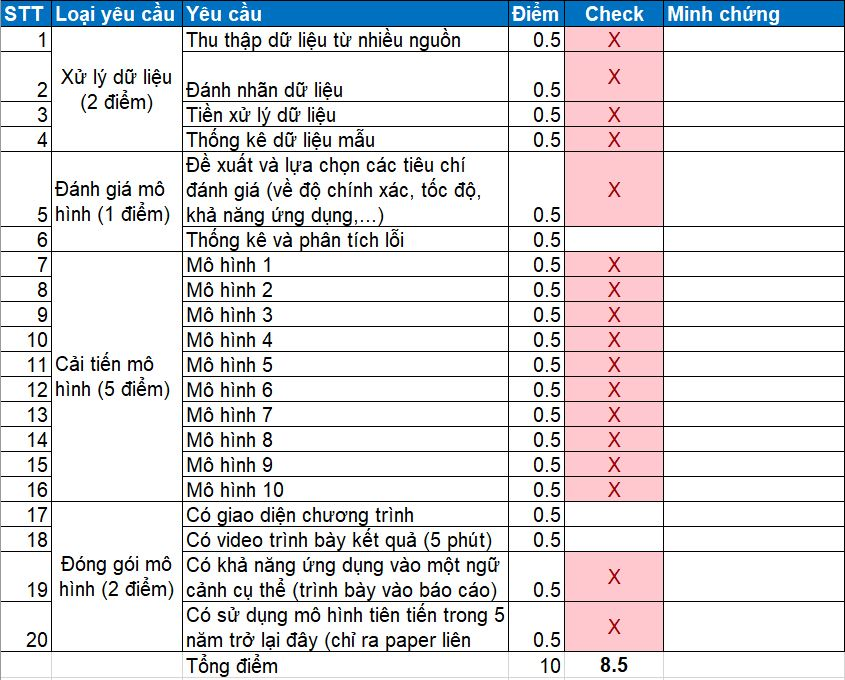
\includegraphics[scale = 1]{fileanh/yeucau.jpg}
        \caption{Checklist}
    \end{figure}
\end{center}

\newpage
\section{Đặt vấn đề}
Ngày nay, xử lý ảnh đang là một lĩnh vực mà rất nhiều người quan tâm và nghiên cứu. Nhờ vào sự phát triển mạnh mẽ của Machine Learning - một lĩnh vực nhỏ của Khoa Học Máy Tính, nó có khả năng tự học hỏi dựa trên dữ liệu đưa vào mà không cần phải được lập trình cụ thể, xử lý ảnh đã và đang được ứng dụng vào nhiều lĩnh vực trong cuộc sống: y tế (X Ray Imaging, PET scan,...), thị giác máy tính (giúp máy tính có thể hiểu, nhận biết đồ vật như con người), các công nghệ nhận dạng (vân tay, khuôn mặt,…)\\

Hiện nay, do sự phát triển của các trang thương mại điện tử - nơi diễn ra sự trao đổi hàng hóa (ví dụ như Shoppe, Lazada,...) ngày càng lớn mạnh nên việc đăng tải các hình ảnh, thông tin của các sản phẩm lên các trang thương mại điện tử đó ngày một phổ biến làm cho lượng dữ liệu trên đó càng trở nên khổng lồ. Chính vì vậy, việc nhận biết và phân loại các sản phẩm đó giúp chúng ta khi muốn tìm kiếm một sản phẩm nào đó dễ dàng hơn.\\     

Các sản phẩm về thời trang như quần áo, giày dép, phụ kiện,... là các sản phẩm hết sức thông dụng trong đời sống con người nên lượng thông tin về các sản phẩm này cũng hết sưc phong phú.Vì thế, việc nhận biết và phân loại các sản phẩm về mặt thời trang cũng có thể coi là một việc cần thiết.\\

\begin{block}{Bài toán}
\begin{itemize}
    \item Input: 
    \begin{itemize}
        \item Hình ảnh của các sản phẩm về thời trang như áo thun, giày, ví, ...
        \item Thông tin của các sản phẩm trên được lưu trong 1 file csv
    \end{itemize}

    \item Bài toán gồm có 3 class: Apparel, Accessories, Footwear

    \item Output: Hệ thống nhận diện và phân loại hình ảnh thuộc lĩnh vực thời trang có khả năng đưa ra được kết quả dự đoán xem hình ảnh đó thuộc class nào.
\end{itemize}
\end{block}
\newpage
\section{Xử lý dữ liệu}
\subsection{Mô tả dữ liệu}
\begin{itemize}
    \item Bộ dữ liệu: Fashion Product Images (Small)
    \item Độ lớn: 593MB
    \item Mô tả: Chứa các hình ảnh thuộc về lĩnh vực thời trang như quần áo, phụ kiện, giày dép
    \item Được lấy trên Kaggle : \href{https://www.kaggle.com/datasets/paramaggarwal/fashion-product-images-small}{https://www.kaggle.com/datasets/paramaggarwal/fashion-product-images-small}
    \item Bộ dữ liệu gồm có:
    \begin{itemize}
        \item Hơn 44000 hình ảnh sản phẩm:
        \begin{itemize}
            \item Có cùng kích thước là 60x80
            \item Tên của mỗi hình ảnh đó chính là cái để xác định thông tin của nó trong file nhãn dữ liệu.
        \end{itemize}
        \begin{center}
            \begin{figure}[!h]
                \centering
                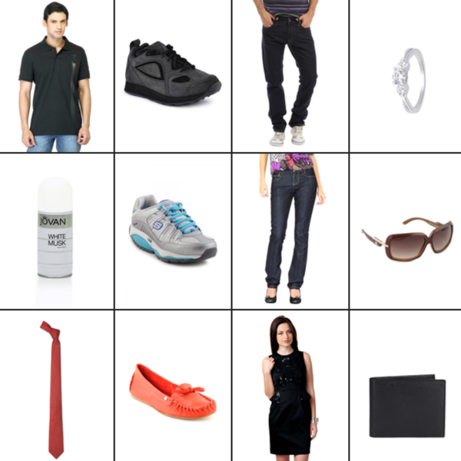
\includegraphics[scale = 0.9]{fileanh/43.png}
                \caption{Hình ảnh sản phẩm}
            \end{figure}
        \end{center}
        \newpage

        \item File nhãn dữ liệu : \textbf{styles.csv}
        \begin{center}
            \begin{figure}[!h]
                \centering
                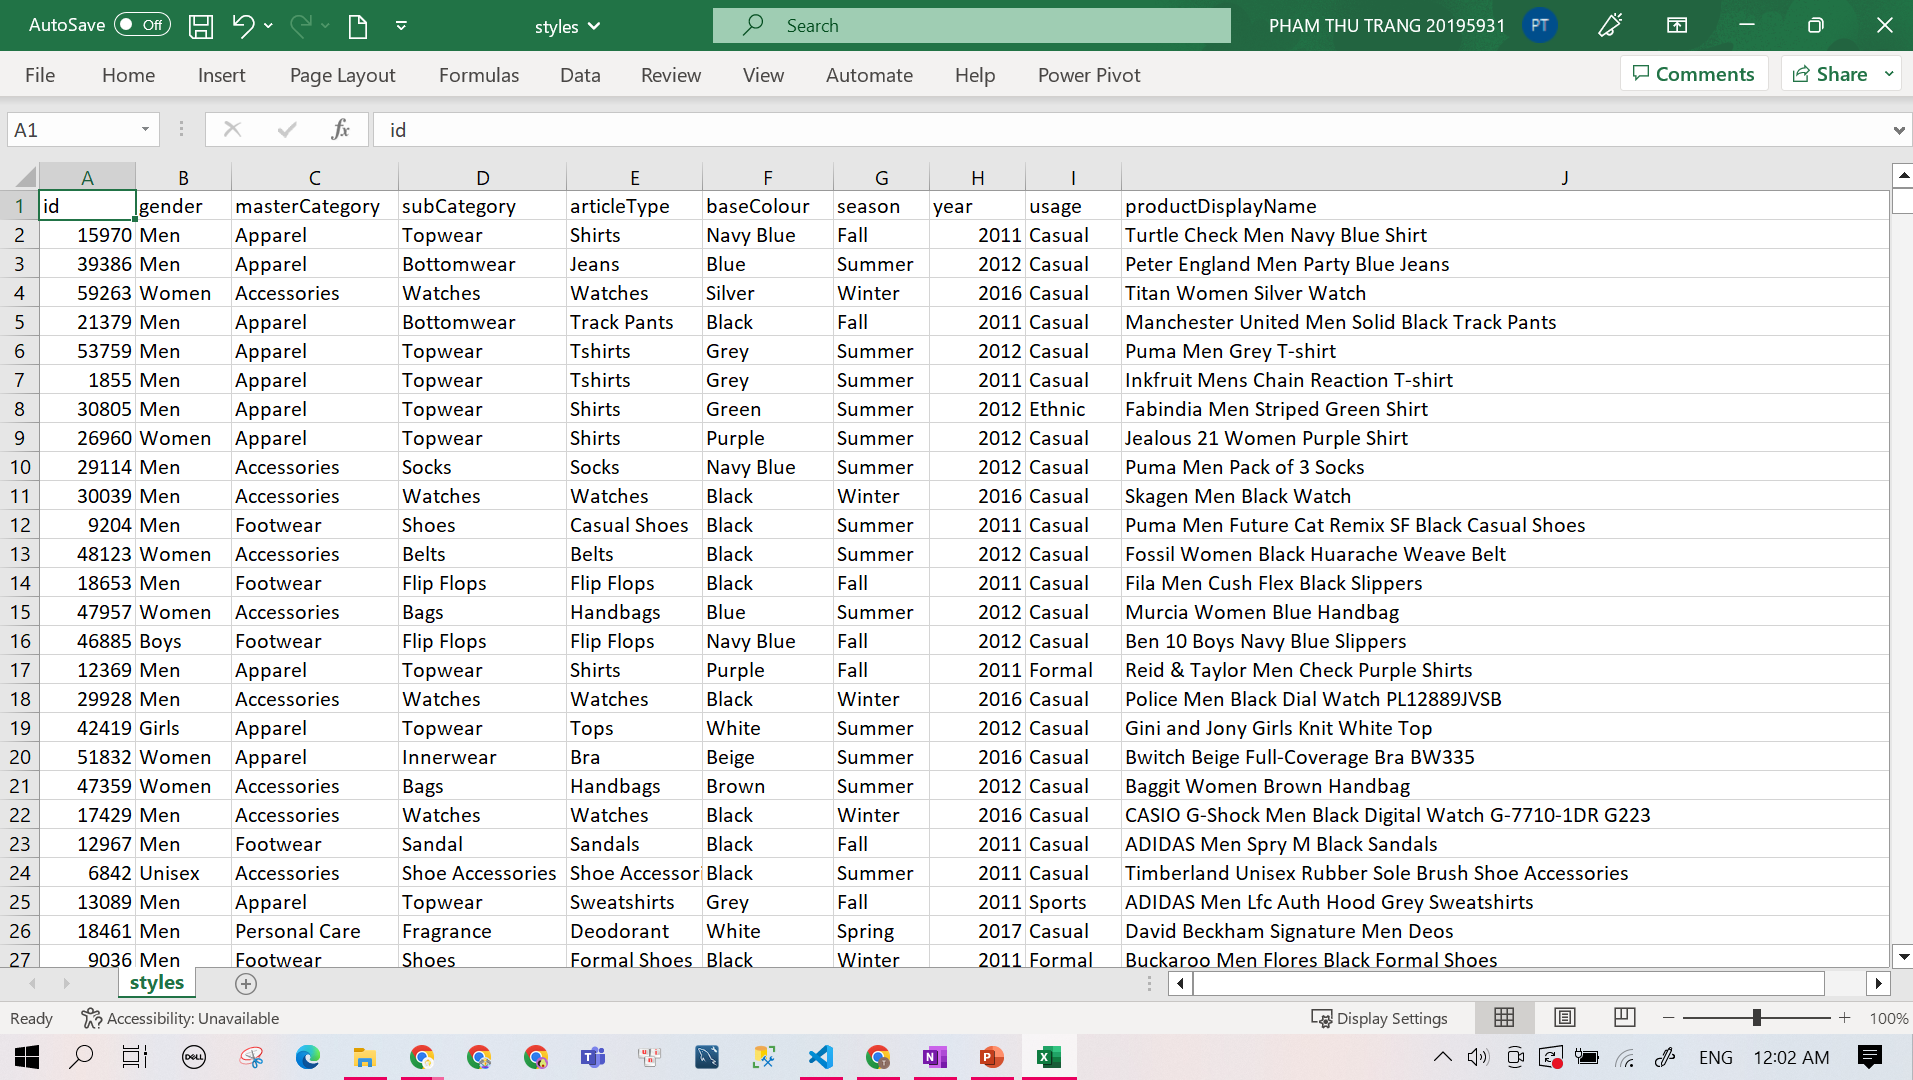
\includegraphics[scale = 0.25]{fileanh/1.png}
                \caption{Bảng mô tả thông tin các hình ảnh}
            \end{figure}
        \end{center}

        \item Hình ảnh trực quan
        \begin{center}
            \begin{figure}[!h]
                \centering
                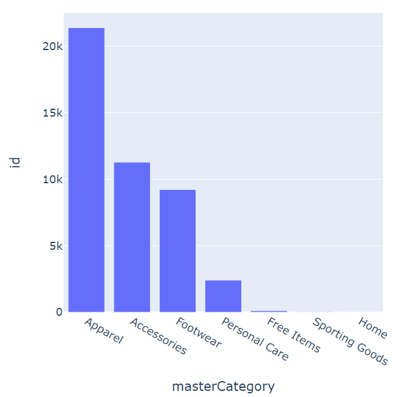
\includegraphics[scale = 0.9]{fileanh/2.png}
                \caption{Số lượng mỗi thuộc tính của cột masterCategory}
            \end{figure}
        \end{center}
        \newpage
        \begin{center}
            \begin{figure}[!h]
                \centering
                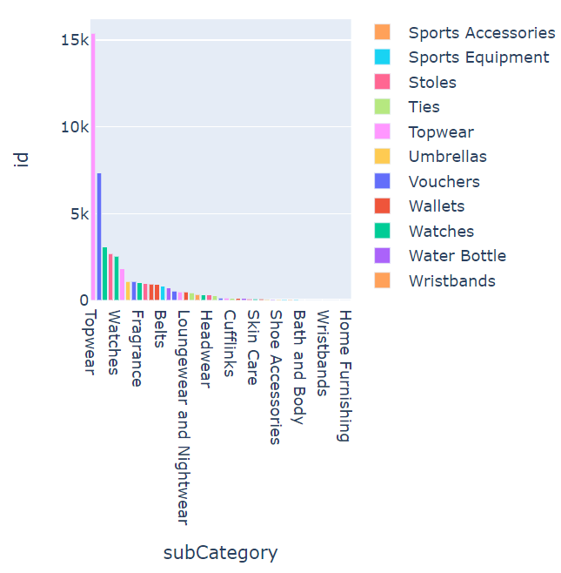
\includegraphics[scale = 1]{fileanh/3.png}
                \caption{Số lượng mỗi thuộc tính của cột subCategory}
            \end{figure}
        \end{center}
        
    \end{itemize}
\end{itemize}

\newpage
\subsection{Tiền xử lý dữ liệu}
Thuộc tính \textbf{masterCategory} gồm có 7 lớp, cụ thể:
\begin{center}
            \begin{figure}[!h]
                \centering
                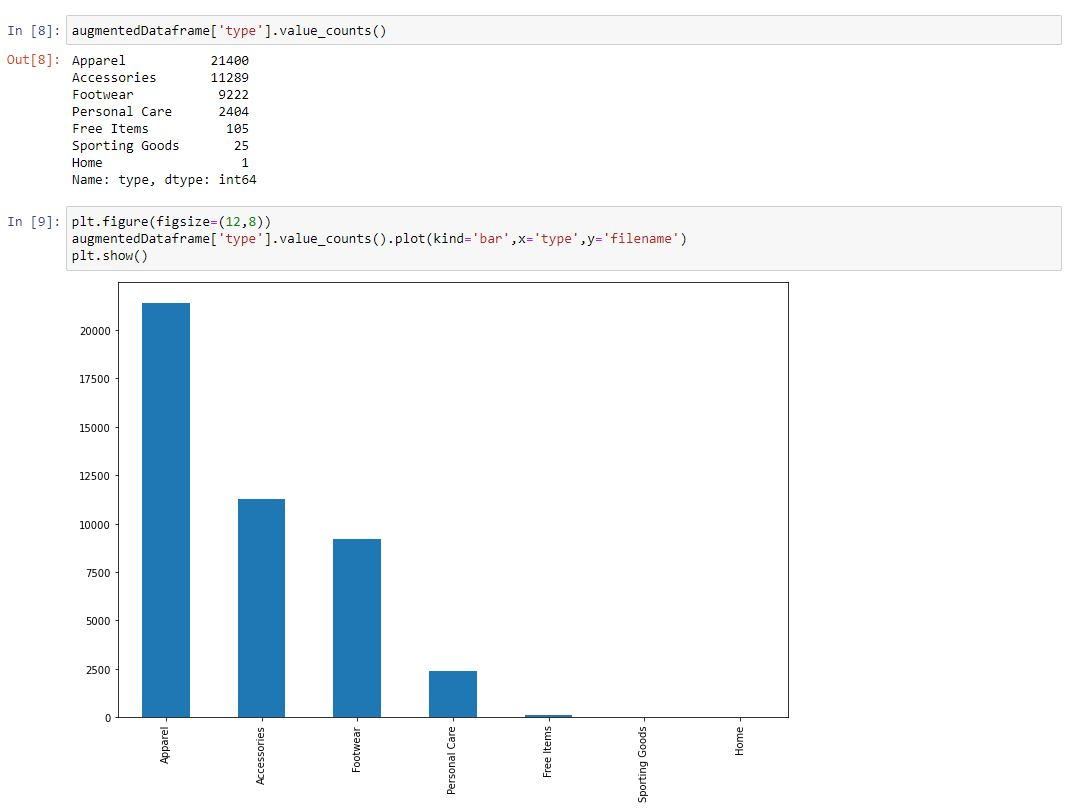
\includegraphics[scale = 0.85]{fileanh/4.jpg}
                \caption{Thông tin của cột masterCategory}
            \end{figure}
        \end{center}
\begin{remark}
    Một số lớp có số lượng quá ít nên sẽ bị loại bỏ và sẽ chỉ giữ lại 3 lớp có số lượng cao nhất trở thành 3 lớp chính cho bài toán.
\end{remark}

\subsubsection{Loại bỏ các lớp không sử dụng}
\begin{lstlisting}[language = python]
data = df.copy()
for i in range(0,total_row,1):
  if df['masterCategory'][i] == 'Personal Care':
    data = data.drop(labels = i, axis =0 )
    os.remove(DATASET_PATH+list_directory[index]+"/"+df.loc[i,'image'])
  elif df['masterCategory'][i] == 'Free Items':
    data = data.drop(labels = i, axis =0 )
    os.remove(DATASET_PATH+list_directory[index]+"/"+df.loc[i,'image'])
  elif df['masterCategory'][i] == 'Sporting Goods':
    data = data.drop(labels = i, axis =0 )
    os.remove(DATASET_PATH+list_directory[index]+"/"+df.loc[i,'image'])
  elif df['masterCategory'][i] =='Home':
    data = data.drop(labels = i, axis =0 )
    os.remove(DATASET_PATH+list_directory[index]+"/"+df.loc[i,'image'])
\end{lstlisting}

\subsubsection{Kiểm tra số lượng hình ảnh và kích thước của dataframe}
\begin{lstlisting}[language = python]
data_path = "C:/Users/admin/3D Objects/Khaiphadulieu/archive/myntradataset/images"
print(len(os.listdir(data_path)))
\end{lstlisting}
41906

\begin{lstlisting}[language = python]
data.shape
\end{lstlisting}
(41911, 11)

\begin{remark}
Số lượng hình ảnh hiện có và số lượng dòng thông tin của các ảnh trong file nhãn là khác nhau.
\end{remark}


\subsubsection{Thống nhất số lượng hình ảnh với file nhãn}
Danh sách các hình ảnh bị thừa/thiếu
\begin{lstlisting}[language = python]
#Su dung khi file anh > so row trong styles.csv
#for i in range(0,total,1):
#  if os.listdir(data_path)[i] not in listt :
#    path = DATASET_PATH+list_directory[index]+"/"+os.listdir(data_path)[i]    
#    shutil.move(path,'C:/Users/admin/3D Objects/Khaiphadulieu/archive/')


#Su dung khi file anh < so row trong styles.csv
path_del = []
for i in range(0,total,1):
    if listt[i] not in os.listdir(data_path):
        #print(listt[i])
        path_del.append(listt[i])
print(path_del)
\end{lstlisting}
['39403.jpg', '39410.jpg', '39401.jpg', '39425.jpg', '12347.jpg']\\

Xóa các dòng trong file nhãn bị thừa
\begin{lstlisting}[language = python]
for i in path_del:
    data = data.drop(data[data['image'] == i].index)
data.shape
\end{lstlisting}
(41906, 11)

\subsubsection{Kết quả thu được}
\begin{lstlisting}[language = python]
data['masterCategory'].value_counts()
\end{lstlisting}
Apparel    \ \ \ \ \ \ \ \ \ \ 21395\\
Accessories \   11289\\
Footwear    \ \ \ \ \ \  9222\\
Name: type, dtype: int64
\newpage
\begin{center}
    \begin{figure}[!h]
        \centering
        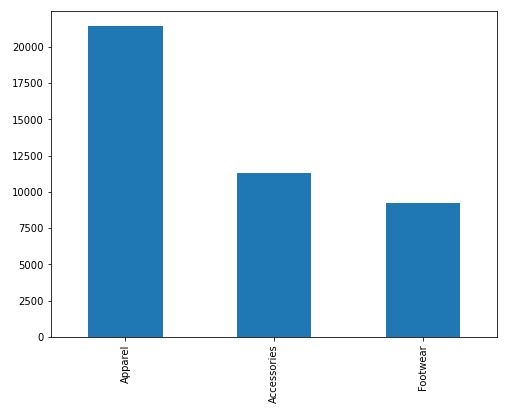
\includegraphics[scale = 1.5]{fileanh/5.jpg}
        \caption{Số lượng mỗi lớp sau khi xử lý}
    \end{figure}
\end{center}

\begin{block}{Nhận xét}
Bài toán này sẽ gồm có:
\begin{itemize}
    \item 41906 hình ảnh đã được gán nhãn 
    \item 3 lớp chính với số lượng như sau:
    \begin{itemize}
        \item Apparel \ \ \ \ \ \ \ 21395
        \item Accessories \ \ 11289
        \item Footwear \ \ \ \ \ \ \ 9222
    \end{itemize}
\end{itemize}
\end{block}
\newpage
\newpage
\section{Tăng cường dữ liệu từ nhiều nguồn}
\subsection{Các nguồn dữ liệu}
\subsubsection{Clothing dataset}
\begin{itemize}
    \item Gồm có 5762 hình ảnh với các kích thước khác nhau.
    \item Độ lớn : 153MB
    \item Mô tả: Đa số là hình ảnh về quần áo, một số ít còn lại là hình ảnh của mũ và giày.
    \item Được lấy trên Kaggle: \href{https://www.kaggle.com/datasets/agrigorev/clothing-dataset-full}{https://www.kaggle.com/datasets/agrigorev/clothing-dataset-full}
\end{itemize}
\begin{center}
    \begin{figure}[!h]
       \centering
       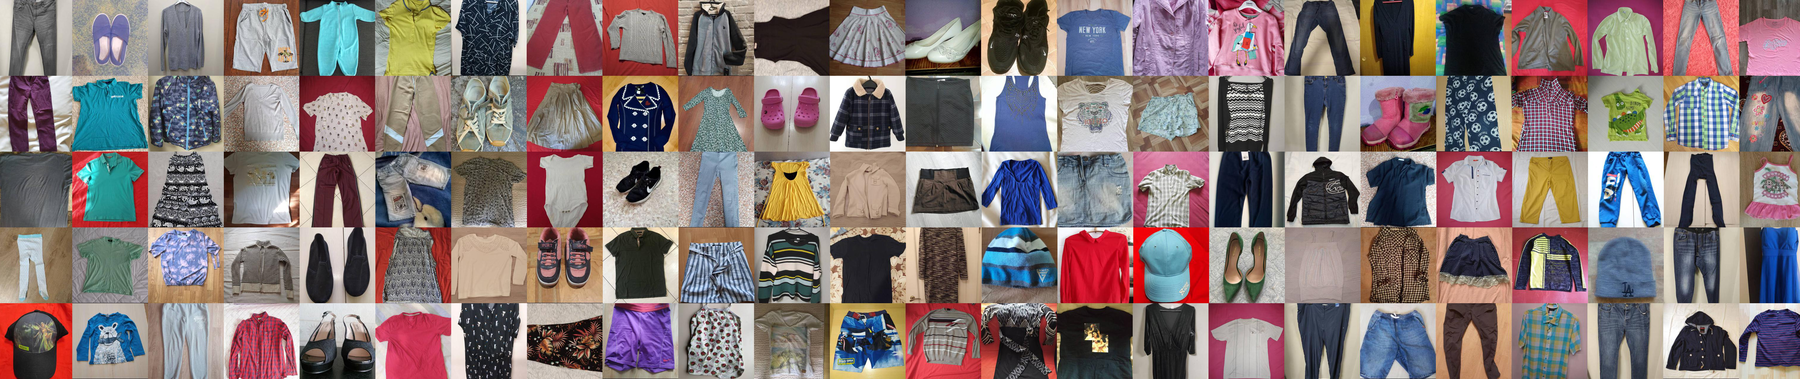
\includegraphics[scale = 0.25]{fileanh/44.png}
     \end{figure}
\end{center}

\subsubsection{Apparel images dataset}
\begin{itemize}
    \item Gồm có 11385 hình ảnh với các kích thước khác nhau.
    \item Độ lớn: 259MB
    \item Mô tả: Các hình ảnh được chia vào 1 trong 24 thư mục tùy thuộc vào mỗi loại và nàu sắc của đồ vật trong ảnh. Gồm hình ảnh về quần áo và giày.
    \item Được lấy trên Kaggle: \href{https://www.kaggle.com/datasets/trolukovich/apparel-images-dataset}{https://www.kaggle.com/datasets/trolukovich/apparel-images-dataset}
\end{itemize}
\begin{center}
    \begin{figure}[!h]
        \centering
        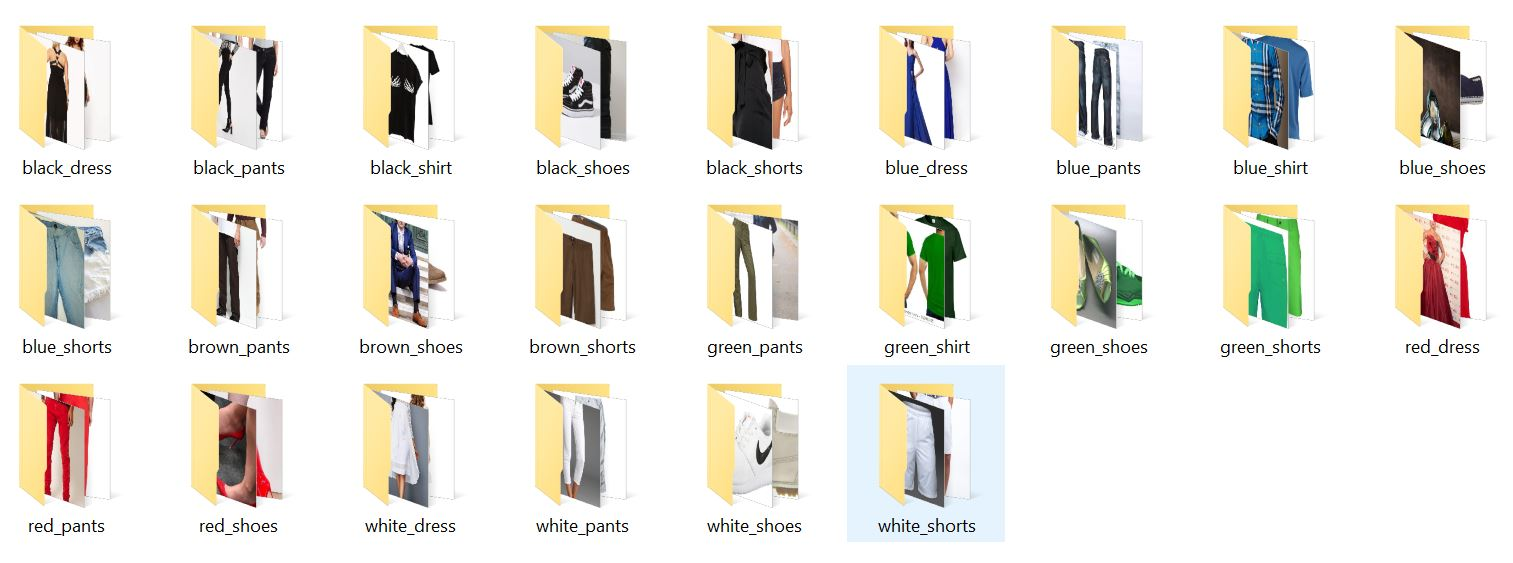
\includegraphics[scale = 0.45]{fileanh/45.jpg}
        \caption{Apparel images dataset}
    \end{figure}
\end{center}


\subsubsection{Shoe vs Sandal vs Boot Image Dataset}
\begin{itemize}
    \item Gồm có 15000 hình ảnh có độ phân giải 136x102 pixel trong mô hình màu RGB.
    \item Độ lớn: 47.4MB
    \item Mô tả: Bộ dữ liệu Hình ảnh Giày vs Sandal vs Boot này chứa 15.000 hình ảnh về giày, dép và bốt. 5000 hình ảnh cho mỗi thể loại. 
    \item Được lấy trên Kaggle: \href{https://www.kaggle.com/datasets/hasibalmuzdadid/shoe-vs-sandal-vs-boot-dataset-15k-images}{https://www.kaggle.com/datasets/hasibalmuzdadid/shoe-vs-sandal-vs-boot-dataset-15k-images}
\end{itemize}
\begin{center}
    \begin{figure}[!h]
        \centering
        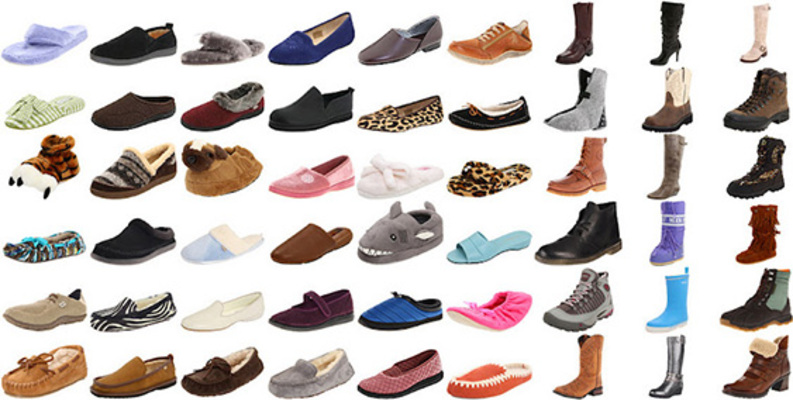
\includegraphics[scale = 1.5]{fileanh/46.jpg}
        \caption{Shoe Dataset}
    \end{figure}
\end{center}

\subsubsection{Một số nguồn dữ liệu khác được sử dụng}
\begin{enumerate}
    \item annotation Image Dataset : \href{https://universe.roboflow.com/honeysys/annotation-uzv7f/dataset/2}{https://universe.roboflow.com/honeysys/annotation-uzv7f/dataset/2}
    \begin{itemize}
        \item Có 2404 hình ảnh về nhẫn (phụ kiện) với cùng kích thước 640x640
        \item Độ lớn : 78.4MB
    \end{itemize}

    \item Bag Image Dataset: \href{https://universe.roboflow.com/bag-va5cg/bag-xbzrp/dataset/1}{https://universe.roboflow.com/bag-va5cg/bag-xbzrp/dataset/1}
    \begin{itemize}
        \item Có 1926 hình ảnh về túi xách (phụ kiện) với các kích thước khác nhau
        \item Độ lớn : 258MB
        
    \end{itemize}

    \item bucket-hats Image Dataset: \href{https://universe.roboflow.com/nathan-vdftz/bucket-hats/dataset/2}{https://universe.roboflow.com/nathan-vdftz/bucket-hats/dataset/2}
    \begin{itemize}
        \item Có 769 hình ảnh về mũ (phụ kiện) với các kích thước khác nhau
        \item Độ lớn : 21.2MB
      
    \end{itemize}

    \item yolo Image Dataset: \href{https://universe.roboflow.com/new-workspace-7lsw2/yolo-w9gld/dataset/2}{https://universe.roboflow.com/new-workspace-7lsw2/yolo-w9gld/dataset/2}
    \begin{itemize}
        \item Có 444 hình ảnh về mũ (phụ kiện) với với cùng kích thước 416x416
        \item Độ lớn : 4.48MB
      
    \end{itemize}
    
\end{enumerate}


\newpage
\subsection{Gán nhãn dữ liệu}
\subsubsection{Đổi tên cho hình ảnh}
Dưới đây là ví dụ cho tập dữ liệu Clothing dataset:
\begin{lstlisting}
for i, filename in enumerate(os.listdir(dataset_path)):
    i += 60001
    dst = f"{str(i)}.jpg"
    src =f"{dataset_path}{filename}"
    dst =f"{dataset_path}{dst}"
    os.rename(src, dst)
\end{lstlisting}
\begin{center}
    \begin{figure}[!h]
        \centering
        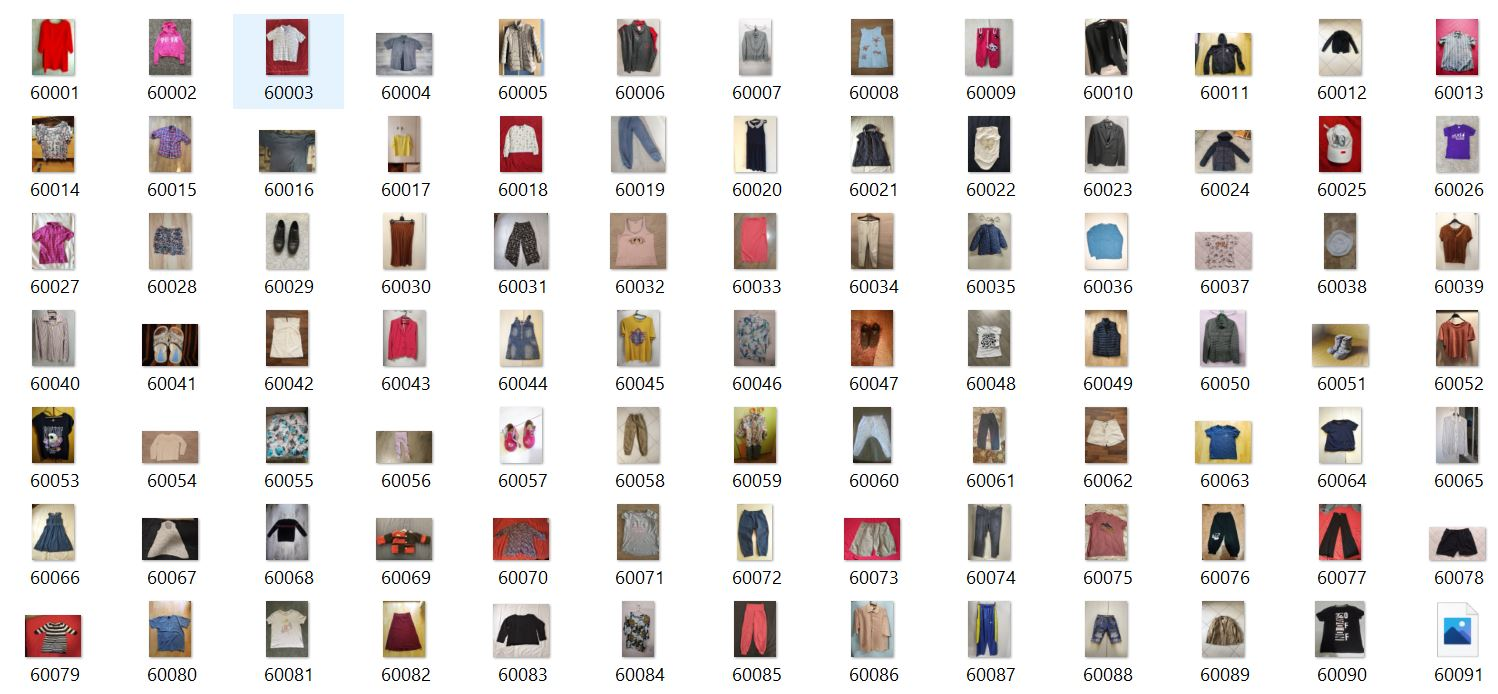
\includegraphics[scale = 0.6]{fileanh/47.jpg}
        \caption{Clothing dataset được đổi tên}
    \end{figure}
\end{center}
\begin{cy}
Các bộ dữ liệu khác làm tương tự.
\end{cy}


\subsubsection{Tạo nhãn cho từng bộ dữ liệu}
Do bộ dữ liệu \textbf{Clothing dataset} chứa tất cả hình ảnh của 3 lớp trong cùng 1 thư mục nên trước khi tạo nhãn ta sẽ phân chúng thành 3 thư mục và thực hiện đoạn code sau:
\begin{lstlisting}
app_path = 'C:/Users/admin/3D Objects/KhaiphaDL_CK/Models/images_compressed/Apparel/'
app = []
for img in os.listdir(app_path):   
    app.append([int(img[:5]), 'Apparel', img])
    
df_app = pd.DataFrame(app, columns = col_names)

acc_path = 'C:/Users/admin/3D Objects/KhaiphaDL_CK/Models/images_compressed/Accessories/'
acc = []
for img in os.listdir(acc_path):   
    acc.append([int(img[:5]), 'Accessories', img])
    
df_acc = pd.DataFrame(acc, columns = col_names)

foot_path = 'C:/Users/admin/3D Objects/KhaiphaDL_CK/Models/images_compressed/Footwear/'
foot = []
for img in os.listdir(foot_path):   
    foot.append([int(img[:5]), 'Footwear', img])
    
df_foot = pd.DataFrame(foot, columns = col_names)

df_app = df_app.append(df_acc,ignore_index = True)
df_app = df_app.append(df_foot,ignore_index = True)
df_app
\end{lstlisting}
\begin{center}
    \begin{figure}[!h]
        \centering
        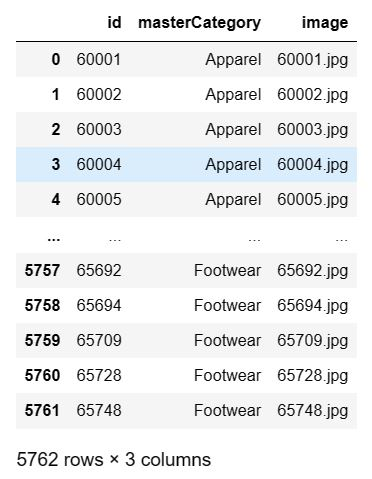
\includegraphics[scale = 1.4]{fileanh/48.jpg}
        \caption{Nhãn của Clothing dataset}
    \end{figure}
\end{center}
\begin{cy}
Các bộ dữ liệu còn lại đều đã được phân lớp thành các thư mục khác nhau hoặc chỉ có 1 lớp duy nhất nên sẽ chỉ cần tạo nhãn theo đúng thư mục tương ứng với lớp của nó.
\end{cy}
\newpage
\subsubsection{Tổng hợp dữ liệu}
\begin{enumerate}
    \item Hình ảnh: thực hiện chuyển hình ảnh của tất cả các bộ dữ liệu về thư mục './myntradataset/images' (thư mục chứa dữ liệu gốc được xử lý phía trên)

    \item Nhãn: Thực hiện tổng hợp lại nhãn của tất cả bộ dữ liệu cả gốc (\textbf{Fashion Product Images (Small)})và tăng cường thêm.
\end{enumerate}

\begin{center}
    \begin{figure}[!h]
        \centering
        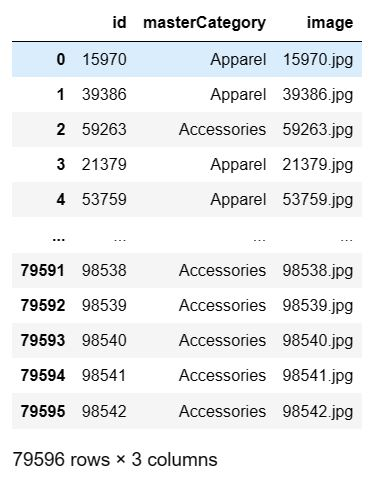
\includegraphics[scale = 1.4]{fileanh/49.jpg}
        \caption{Nhãn cho dữ liệu sau khi tăng cường}
    \end{figure}
\end{center}

\subsubsection{Kết quả thu được }
\begin{lstlisting}[language = python]
df_main['masterCategory'].value_counts()
\end{lstlisting}
Apparel    \ \ \ \ \ \ \ \ \ \ 34452\\
Accessories \   17033\\
Footwear    \ \ \ \ \ \  28111\\
Name: type, dtype: int64
\newpage
\begin{center}
    \begin{figure}[!h]
        \centering
        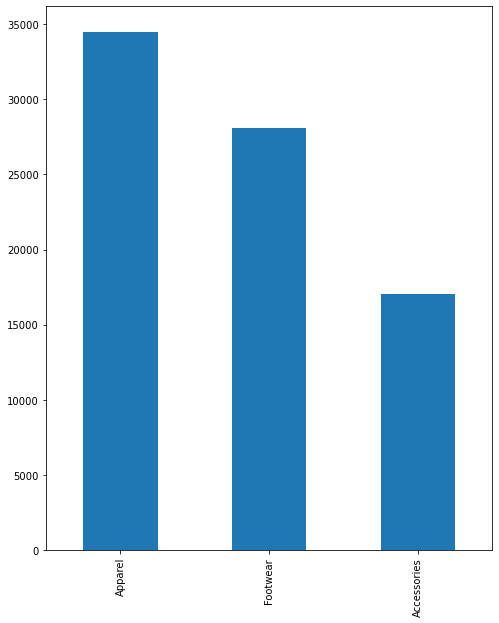
\includegraphics[scale = 0.6]{fileanh/50.png}
        \caption{Số lượng mỗi lớp sau khi tăng cường}
    \end{figure}
\end{center}

\begin{block}{Nhận xét}
Bài toán hiện tại sẽ gồm có:
\begin{itemize}
    \item 79596 hình ảnh đã được gán nhãn 
    \item 3 lớp chính với số lượng như sau:
    \begin{itemize}
        \item Apparel \ \ \ \ \ \ \ 34452
        \item Accessories \ \ 17033
        \item Footwear \ \ \ \ \ \ \ 28111
    \end{itemize}
\end{itemize}
\end{block}
\newpage
\section{Đánh giá mô hình}
%\subsection{Confusion matrix}
\textbf{Confusion matrix} (ma trận nhầm lẫn hay ma trận lỗi) là một trong các kỹ thuật tính toán hiệu suất thường được sử dụng trong các bài toán phân loại.\\

Với bài toán đang xét gồm có 3 lớp thì ta có ma trận nhầm lẫn cho 3 lớp ví dụ như hình sau:
\begin{center}
    \begin{figure}[!h]
        \centering
        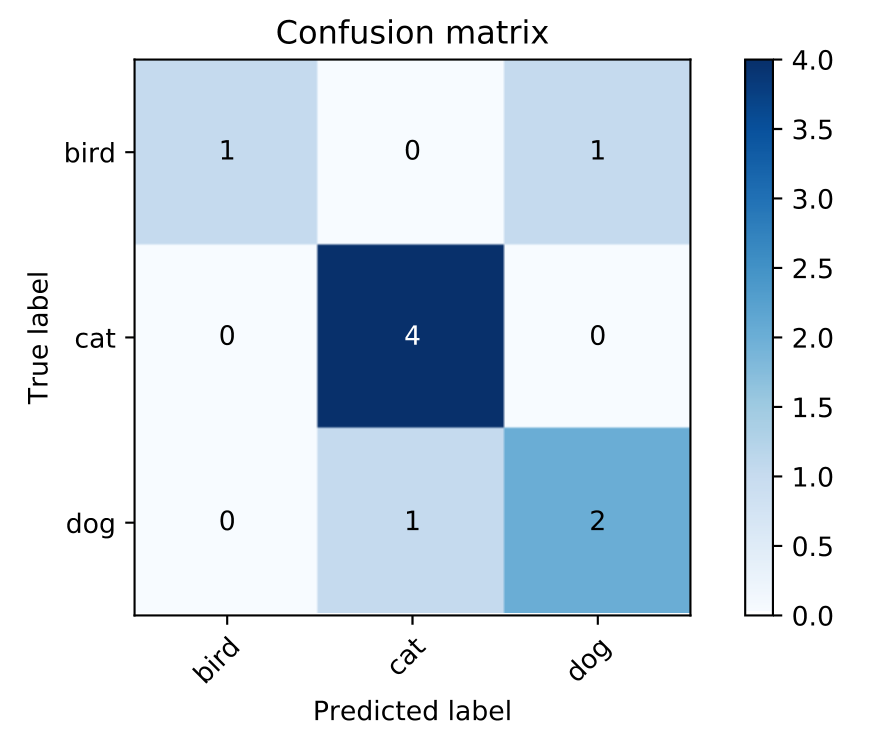
\includegraphics[scale = 0.5]{fileanh/6.png}
        \caption{confusion matrix}
    \end{figure}
\end{center}
Ví dụ ta xét lớp \textbf{Birt} thì True Positives (TP), False Positives (FP), False Negatives (FN) và True Negatives (TN) sẽ được xác định
\begin{center}
    \begin{figure}[!h]
        \centering
        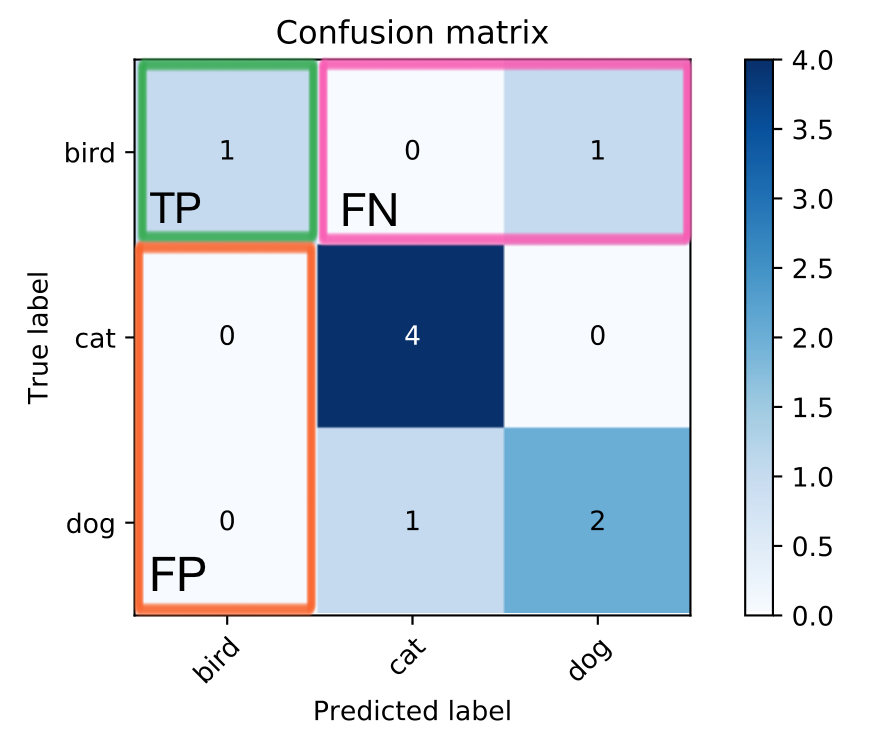
\includegraphics[scale = 0.5]{fileanh/7.png}
        \caption{Xác định TP, FP, FN cho lớp Birt}
    \end{figure}
\end{center}
True Negatives (TN) sẽ được hiểu các ô còn lại trong đó. Từ đây ta có:
\begin{itemize}
    \item True Positives (TP): là giá trị của ô vuông có tên của nhãn thực sự và nhãn dự đoán trùng nhau.
    \item False Positives (FP): là giá trị của 2 ô còn lại xét theo cột nhãn dự đoán của lớp cần tìm.
    \item False Negatives (FN): là giá trị của 2 ô còn lại xét theo cột nhãn thực sự của lớp cần tìm.
    \item True Negatives (TN): là giá trị của các ô còn lại.
\end{itemize}
Cuối cùng thu được bảng kết quả:
\begin{center}
    \begin{figure}[!h]
        \centering
        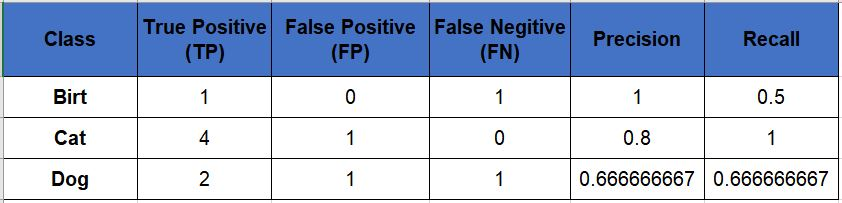
\includegraphics[scale = 1]{fileanh/8.jpg}
        \caption{Xác định TP, FP, FN cho lớp Birt}
    \end{figure}
\end{center}
Trong đó:
$\displaystyle \text{Precision}\ = \frac{TP}{TP + FP},\ \text{ Recall}\ = \frac{TP}{TP + FN}$\\

\textbf{Macro average precision} (Độ chính xác trung bình vĩ mô) là giá trị trung bình của tất cả các Precision của mỗi lớp.
$$\text{PrecisionMacroAvg}\ = \frac{Prec_1 + Prec_2 + \cdots + Prec_n}{n}$$
Xét ví dụ trên, có:
$$\text{PrecisionMacroAvg}\ = \frac{Prec_{Birt} + Prec_{Cat} + Prec_{Dog}}{3} = \frac{1 + 0.8+0.6667}{3} = 0.8222$$


\textbf{Macro average recall} (Khả năng thu hồi trung bình vĩ mô) là giá trị trung bình cộng của tất cả các Recall của mỗi lớp.
$$\text{RecallMacroAvg}\ = \frac{Recall_1 + Recall_2 + \cdots + Recall_n}{n}$$
Xét ví dụ trên, có:
$$\text{RecallMacroAvg}\ = \frac{Recall_{Birt} + Recall_{Cat} + Recall_{Dog}}{3} = \frac{0.5 + 1+0.6667}{3} = 0.7222$$


\textbf{F1-score} - điểm F cân bằng hay thước đo F có thể hiểu là trung bình điều hòa của độ chính xác (precision) và khả năng thu hồi (recall).
$$F_1 = \frac{2*(Precision * Recall)}{Precision + Recall}$$
\newpage
\section{Cải tiến mô hình}
\subsection{Mô hình 1 - CNN}
\subsubsection{Dữ liệu đầu vào }
Mô hình này sẽ có đầu vào là bộ dữ liệu \textbf{Fashion Product Images (Small)} đã được xử lý với 41906 hình ảnh cho 3 lớp.\\

Sử dụng \textbf{ImageDataGenerator} chia dữ liệu thành 2 tập là training\_generator và validation\_generator, đồng thời tăng cường thêm dữ liệu như sau:
\begin{lstlisting}
from keras.preprocessing.image import ImageDataGenerator

#image generator object from keras. reference : Keras Docs
image_generator = ImageDataGenerator(
    validation_split=0.2, 
    rescale=1/255, 
    shear_range = 0.2, 
    zoom_range = 0.2, 
    horizontal_flip = True
)

#create a flow of images for training the model.
training_generator = image_generator.flow_from_dataframe(
    dataframe = df,
    directory= "/content/drive/MyDrive/myntradataset/images/",
    x_col="image",
    y_col="masterCategory",
    target_size=(224,224),
    batch_size=32,
    subset="training"

)

#create a flow of images for validating(testing) the trained model.
validation_generator = image_generator.flow_from_dataframe(
    dataframe = df,
    directory="/content/drive/MyDrive/myntradataset/images/",
    x_col="image",
    y_col="masterCategory",
    target_size=(224,224),
    batch_size=32,
    subset="validation"
)
\end{lstlisting}
Found 33525 validated image filenames belonging to 3 classes.\\
Found 8381 validated image filenames belonging to 3 classes.\\

\newpage
Còn tập test sẽ đc lấy ra một phần từ tập validation\_generator như sau:
\begin{lstlisting}
batch_size = 32
#!pip install tqdm
import tqdm
validation_generator.reset()
X_test, y_test = next(validation_generator)
for i in tqdm.tqdm(range(int(validation_generator.n/batch_size)-200)): 
  img, label = next(validation_generator)
  X_test = np.append(X_test, img, axis=0 )
  y_test = np.append(y_test, label, axis=0)
print(X_test.shape, y_test.shape)
\end{lstlisting}
Thu được tập test gồm có 1984 hình ảnh và nhãn của nó.

\subsubsection{Xây dựng mô hình}
%So với mô hình 1 thì mô hình thứ 2 này tuy vẫn dùng CNN nhưng cấu trúc nó thì được thay đổi, kể cả việc đưa dữ liệu đầu vào cũng đc xử lý theo một cách khác với target\_size là 224
\begin{lstlisting}
from keras import layers,models
model1 = Sequential()
model1.add(layers.Conv2D(16, (4,4),  activation = 'relu' , input_shape = (224,224,3)))
model1.add(MaxPooling2D(pool_size = (2, 2)))

model1.add(Conv2D(32, (3,3), activation='relu'))
model1.add(MaxPooling2D(pool_size = (2, 2)))

model1.add(Conv2D(64, (3,3), activation='relu'))
model1.add(MaxPooling2D(pool_size = (2, 2)))

model1.add(Conv2D(64, (3,3), activation='relu'))
model1.add(MaxPooling2D(pool_size = (2, 2)))

model1.add(Conv2D(128, (3,3), activation='relu'))
model1.add(MaxPooling2D(pool_size = (2, 2)))


model1.add(Flatten())
model1.add(Dense(units=512, activation='relu'))
model1.add(Dropout(0.25))
model1.add(Dense(units=256, activation='relu'))
model1.add(Dropout(0.25))
model1.add(Dense(units=128, activation='relu'))
model1.add(Dropout(0.25))
model1.add(Dense(units=3, activation='softmax'))

model1.compile(optimizer='adam',
              loss='categorical_crossentropy',
              metrics=['accuracy'])

model1.summary()
\end{lstlisting}
\newpage
\begin{center}
    \begin{figure}[!h]
        \centering
        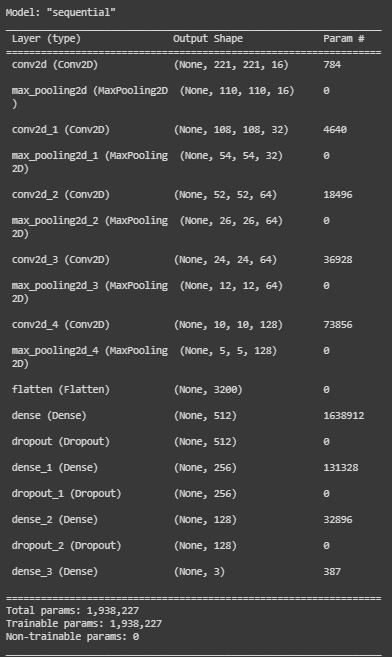
\includegraphics[scale = 1.2]{fileanh/13.jpg}
        \caption{Model CNN}
    \end{figure}
\end{center}
\subsubsection{Kết quả training}
\begin{center}
    \begin{figure}[!h]
        \centering
        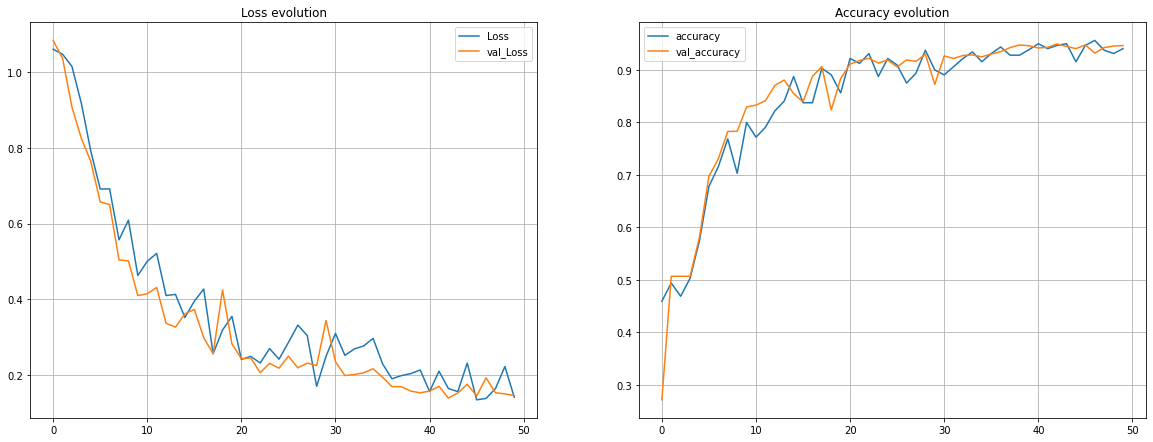
\includegraphics[scale = 0.38]{fileanh/17.png}
        \caption{Kết quả train của Model CNN}
    \end{figure}
\end{center}
\subsubsection{Đánh giá}
Ta có ma trận nhầm lẫn như sau:
\begin{center}
    \begin{figure}[!h]
        \centering
        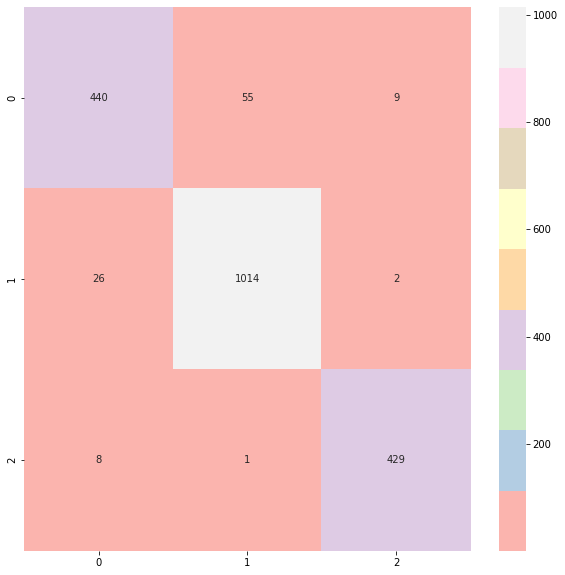
\includegraphics[scale = 0.4]{fileanh/18.png}
        \caption{Confusion matrix của Model CNN}
    \end{figure}
\end{center}
Và các giá trị Macro average Precision, Macro average Recall, F1-score là:
\begin{center}
    \begin{figure}[!h]
        \centering
        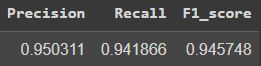
\includegraphics[scale = 1.6]{fileanh/19.jpg}
        \caption{Các chỉ số đánh giá của Model CNN}
    \end{figure}
\end{center}


\subsection{Mô hình 2 - CNN với tập dữ liệu lớn}
Sử dụng mô hình CNN đã được xây dựng trước đó, thực hiện training với tập dữ liệu lớn hơn.
\subsubsection{Dữ liệu đầu vào }
\begin{itemize}
    \item Mô hình này sẽ có đầu vào là bộ dữ liệu đã được tăng cường hình ảnh từ nhiều nguồn khác với tất cả 79596 hình ảnh cho 3 lớp.

    \item Sử dụng \textbf{ImageDataGenerator} thực hiện tăng cường và chia dữ liệu thành các tập train, test và validation với số lượng ảnh gốc (chưa được tăng cường ví dụ như xoay ảnh,..):
    \begin{itemize}
        \item train : 63677 hình ảnh
        \item validation : 15919 hình ảnh
        \item test : 3136 hình ảnh
    \end{itemize}
\end{itemize}

\subsubsection{Kết quả training}
\begin{center}
    \begin{figure}[!h]
        \centering
        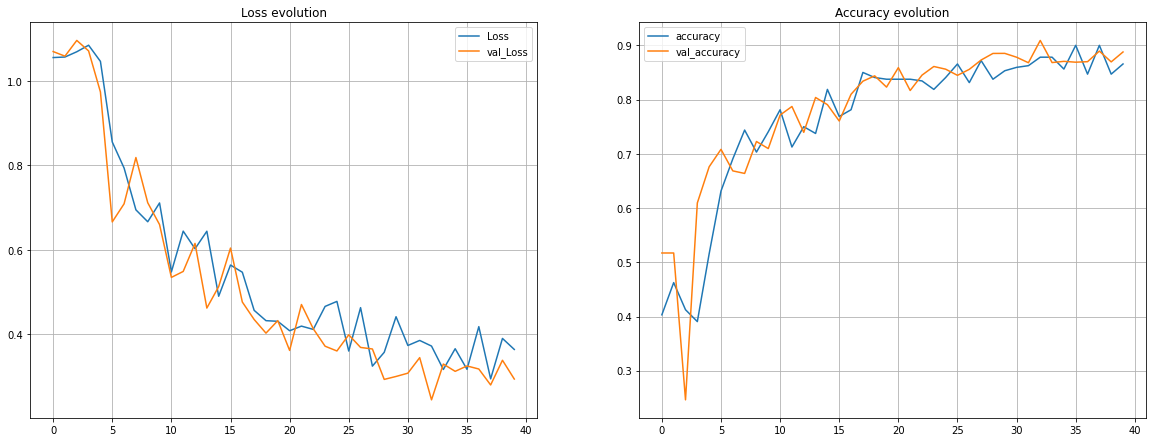
\includegraphics[scale = 0.38]{fileanh/CNNtc.png}
        \caption{Kết quả train của Model CNN với tập dữ liệu lớn}
    \end{figure}
\end{center}
\subsubsection{Đánh giá}
Ta có ma trận nhầm lẫn như sau:
\begin{center}
    \begin{figure}[!h]
        \centering
        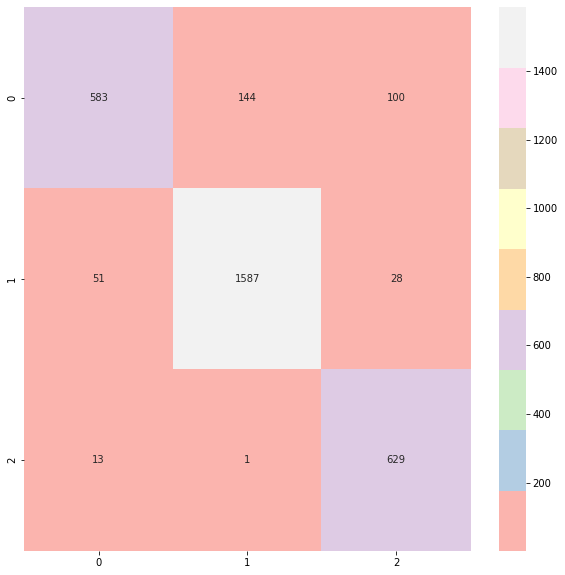
\includegraphics[scale = 0.42]{fileanh/CNNtc1.png}
        \caption{Confusion matrix của Model CNN với tập dữ liệu lớn}
    \end{figure}
\end{center}
\newpage
Và các giá trị Macro average Precision, Macro average Recall, F1-score là:
\begin{center}
    \begin{figure}[!h]
        \centering
        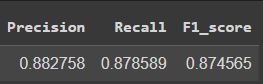
\includegraphics[scale = 1.5]{fileanh/CNNtc2.jpg}
        \caption{Các chỉ số đánh giá của Model CNN với tập dữ liệu lớn}
    \end{figure}
\end{center}

\subsection{Mô hình 3 - VGG16}
\subsubsection{Dữ liệu đầu vào}
Bộ dữ liệu \textbf{Fashion Product Images (Small)} đã được xử lý với 41906 hình ảnh cho 3 lớp.
\subsubsection{Xây dựng mô hình}
\begin{lstlisting}
image_size=[227,227]
model=VGG16(input_shape=image_size+[3],include_top=False,weights="imagenet")
\end{lstlisting}
\begin{lstlisting}
for layers in model.layers:
  layers.trainable=False
\end{lstlisting}
Thêm một số layers cần thiết
\begin{lstlisting}
final_model=Model(inputs=model.input,outputs=Dense(3,activation="softmax")(Flatten()(model.output)))
final_model.summary()
\end{lstlisting}
\begin{lstlisting}
final_model.compile(loss="binary_crossentropy",optimizer="adam",metrics=['accuracy'])  
vgg16=final_model.fit(training_generator,epochs=50,steps_per_epoch=20,validation_data=validation_generator)
\end{lstlisting}
\newpage
\begin{center}
    \begin{figure}[!h]
        \centering
        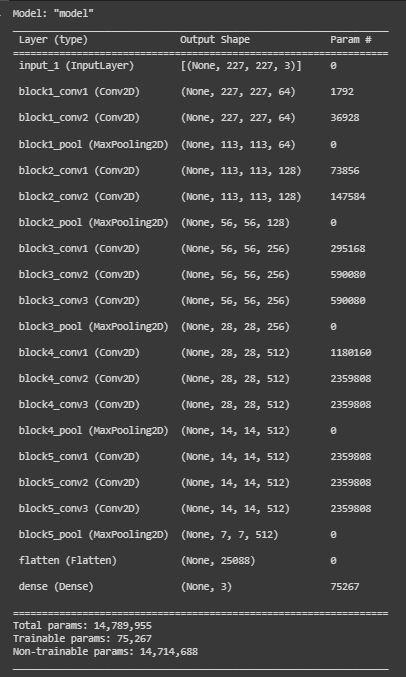
\includegraphics[scale = 1]{fileanh/20.jpg}
        \caption{Model VGG16}
    \end{figure}
\end{center}
\subsubsection{Kết quả training}
\begin{center}
    \begin{figure}[!h]
        \centering
        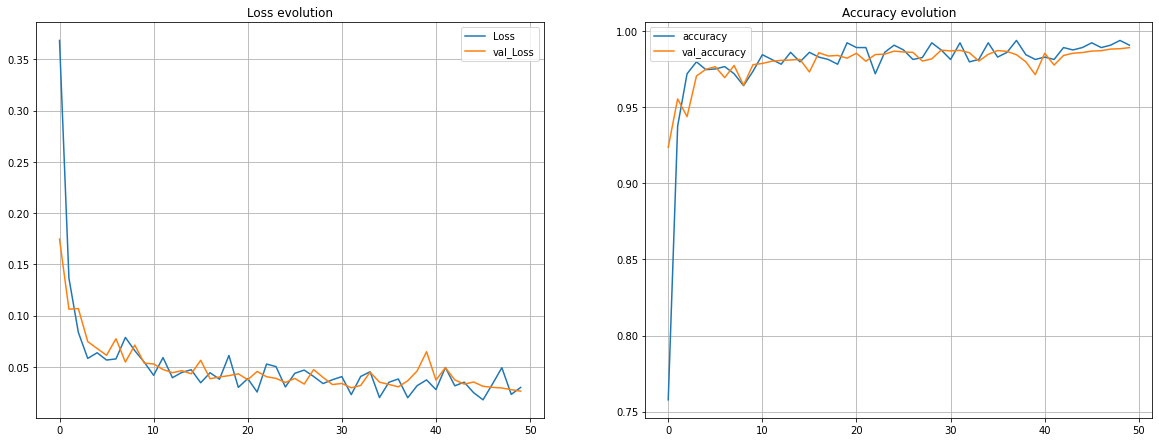
\includegraphics[scale = 0.38]{fileanh/23.png}
        \caption{kết quả train của Model VGG16}
    \end{figure}
\end{center}\newpage
\subsubsection{Đánh giá}
Các giá trị trên ma trận nhầm lẫn:

\begin{center}
    \begin{figure}[!h]
        \centering
        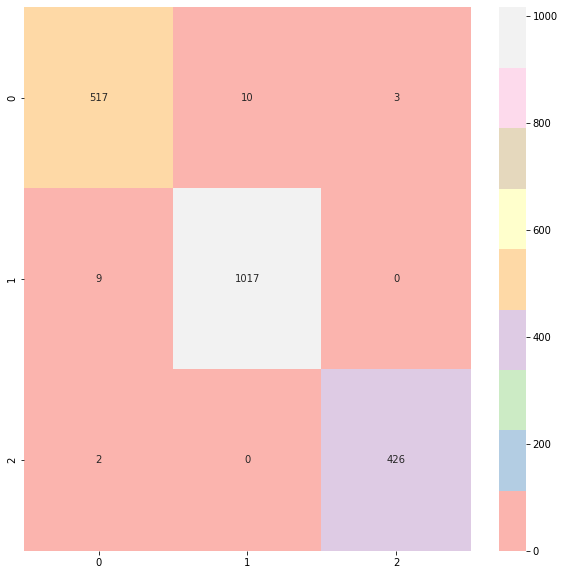
\includegraphics[scale = 0.42]{fileanh/24.png}
        \caption{Confusion matrix của Model VGG16}
    \end{figure}
\end{center}
Và các giá trị Macro average Precision, Macro average Recall, F1-score là:
\begin{center}
    \begin{figure}[!h]
        \centering
        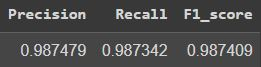
\includegraphics[scale = 1.5]{fileanh/25.jpg}
        \caption{Chỉ số đánh giá của Model VGG16}
    \end{figure}
\end{center}

\subsection{Mô hình 4 - VGG16 với tập dữ liệu lớn}
Sử dụng mô hình VGG16 đã được xây dựng trước đó, thực hiện training với tập dữ liệu lớn hơn.
\subsubsection{Dữ liệu đầu vào }
Bộ dữ liệu đã được tăng cường hình ảnh từ nhiều nguồn khác với tất cả 79596 hình ảnh cho 3 lớp.

\subsubsection{Kết quả training}\newpage
\begin{center}
    \begin{figure}[!h]
        \centering
        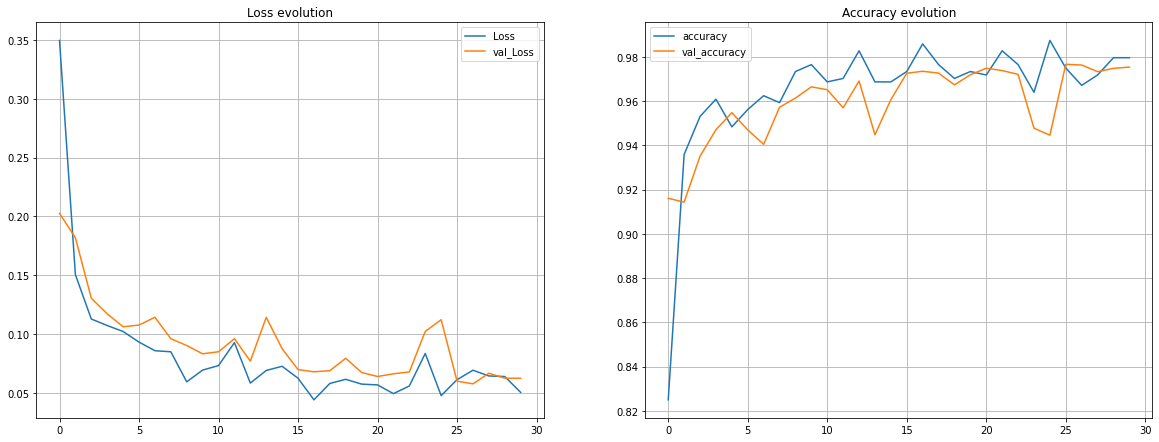
\includegraphics[scale = 0.38]{fileanh/vgg16_increase.png}
        \caption{Kết quả train của Model VGG16 với tập dữ liệu lớn}
    \end{figure}
\end{center}
\subsubsection{Đánh giá}
Ta có ma trận nhầm lẫn như sau:
\begin{center}
    \begin{figure}[!h]
        \centering
        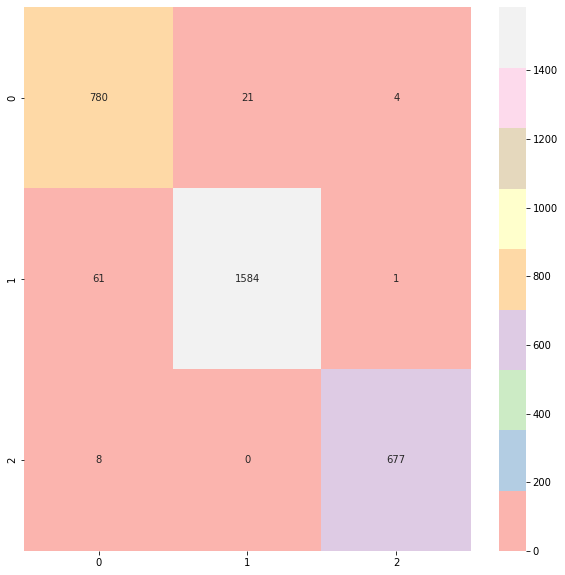
\includegraphics[scale = 0.39]{fileanh/vgg16_increase1.png}
        \caption{Confusion matrix của Model VGG16 với tập dữ liệu lớn}
    \end{figure}
\end{center}

Và các giá trị Macro average Precision, Macro average Recall, F1-score là:
\begin{center}
    \begin{figure}[!h]
        \centering
        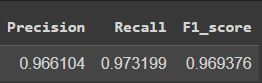
\includegraphics[scale = 1.2]{fileanh/vgg16_increase2.jpg}
        \caption{Các chỉ số đánh giá của Model VGG16 với tập dữ liệu lớn}
    \end{figure}
\end{center}


\subsection{Mô hình 5 - VGG19}
\subsubsection{Dữ liệu đầu vào}
Bộ dữ liệu \textbf{Fashion Product Images (Small)} đã được xử lý với 41906 hình ảnh cho 3 lớp.
\subsubsection{Xây dựng mô hình}
\begin{lstlisting}
image_size=[227,227]
model1=VGG19(input_shape=image_size+[3],include_top=False,weights="imagenet")
\end{lstlisting}
\begin{lstlisting}
for layers in model1.layers:
  layers.trainable=False
\end{lstlisting}
Thêm một số layers cần thiết
\begin{lstlisting}
final_model1=Model(inputs=model1.input,outputs=Dense(3,activation="softmax")(Flatten()(model1.output)))
final_model1.summary()
\end{lstlisting}

\begin{center}
    \begin{figure}[!h]
        \centering
        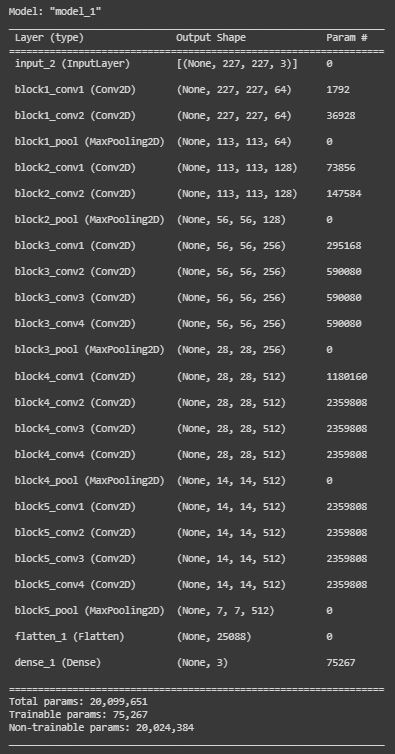
\includegraphics[scale = 1]{fileanh/26.jpg}
        \caption{Model VGG19}
    \end{figure}
\end{center}

\begin{lstlisting}
final_model1.compile(loss="binary_crossentropy",optimizer="adam",metrics=['accuracy'])
vgg19=final_model1.fit(training_generator,epochs=50,steps_per_epoch=20,validation_data=validation_generator)
\end{lstlisting}

\subsubsection{Kết quả training}
\begin{center}
    \begin{figure}[!h]
        \centering
        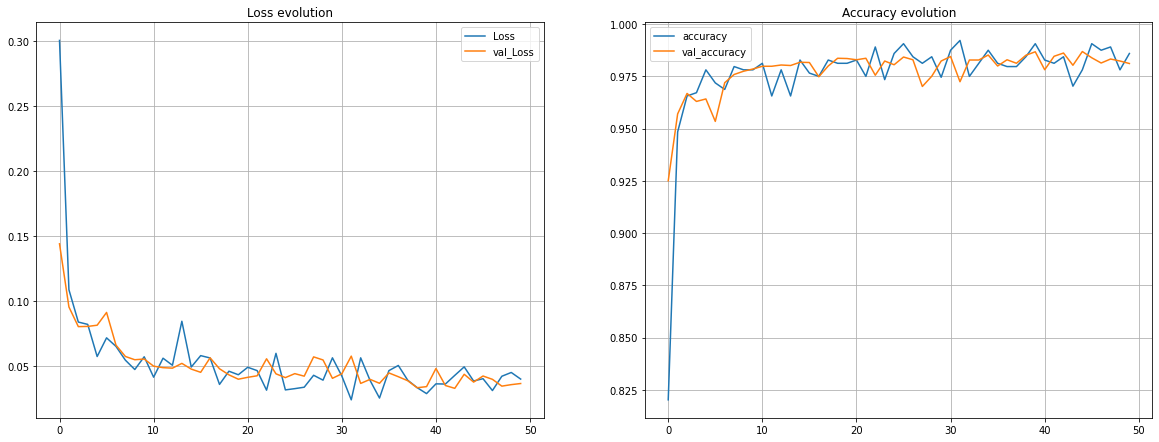
\includegraphics[scale = 0.38]{fileanh/30.png}
        \caption{kết quả train của Model VGG19}
    \end{figure}
\end{center}
\subsubsection{Đánh giá}
Các giá trị trên ma trận nhầm lẫn:
%\newpage
\begin{center}
    \begin{figure}[!h]
        \centering
        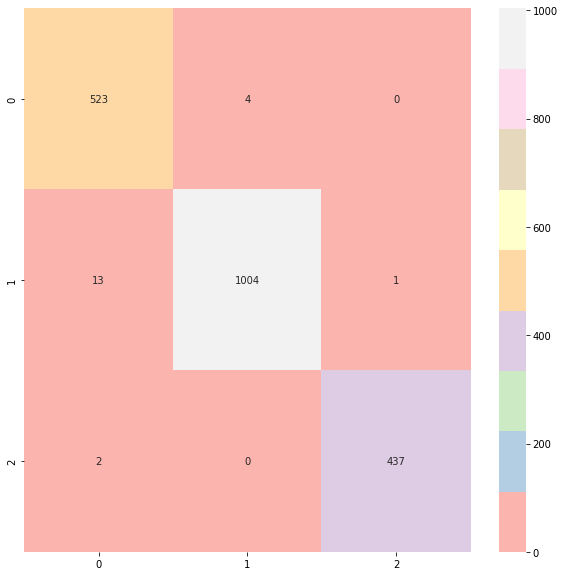
\includegraphics[scale = 0.4]{fileanh/31.png}
        \caption{Confusion matrix của Model VGG19}
    \end{figure}
\end{center}
Và các giá trị Macro average Precision, Macro average Recall, F1-score là:
\begin{center}
    \begin{figure}[!h]
        \centering
        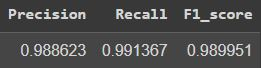
\includegraphics[scale = 1.5]{fileanh/32.jpg}
        \caption{Chỉ số đánh giá của Model VGG19}
    \end{figure}
\end{center}

\subsection{Mô hình 6 - VGG19 với tập dữ liệu lớn}
Sử dụng mô hình VGG19 đã được xây dựng trước đó, thực hiện training với tập dữ liệu lớn hơn.
\subsubsection{Dữ liệu đầu vào }
Bộ dữ liệu đã được tăng cường hình ảnh từ nhiều nguồn khác với tất cả 79596 hình ảnh cho 3 lớp.

\subsubsection{Kết quả training}
\begin{center}
    \begin{figure}[!h]
        \centering
        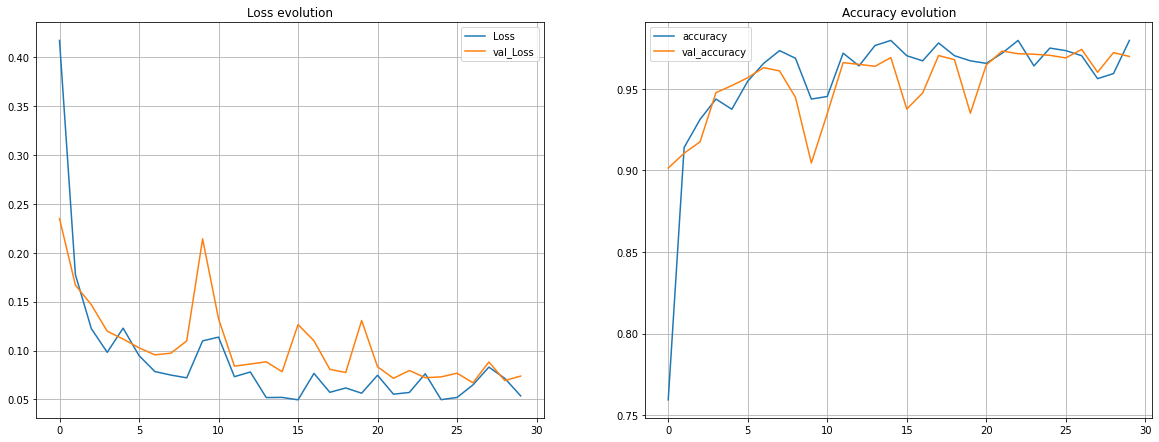
\includegraphics[scale = 0.38]{fileanh/vgg19_increase.png}
        \caption{Kết quả train của Model VGG19 với tập dữ liệu lớn}
    \end{figure}
\end{center}
\subsubsection{Đánh giá}
Ta có ma trận nhầm lẫn như sau:
\begin{center}
    \begin{figure}[!h]
        \centering
        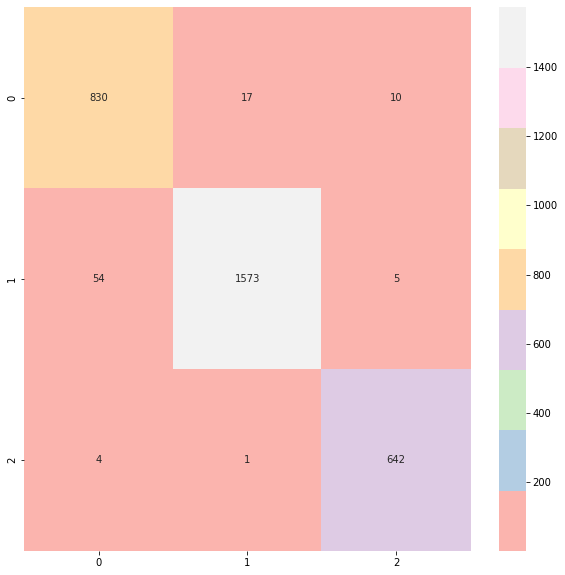
\includegraphics[scale = 0.4]{fileanh/vgg19_increase1.png}
        \caption{Confusion matrix của Model VGG19 với tập dữ liệu lớn}
    \end{figure}
\end{center}
\newpage
Và các giá trị Macro average Precision, Macro average Recall, F1-score là:
\begin{center}
    \begin{figure}[!h]
        \centering
        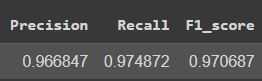
\includegraphics[scale = 1.2]{fileanh/vgg19_increase2.jpg}
        \caption{Các chỉ số đánh giá của Model VGG19 với tập dữ liệu lớn}
    \end{figure}
\end{center}






\subsection{Mô hình 7 - Alexnet}
\subsubsection{Dữ liệu đầu vào}
Bộ dữ liệu \textbf{Fashion Product Images (Small)} đã được xử lý với 41906 hình ảnh cho 3 lớp.
\subsubsection{Xây dựng mô hình}
\begin{lstlisting}
model=Sequential()
model.add(Conv2D(filters=96,strides=(4,4),kernel_size=(11,11),padding='valid',input_shape=(227,227,3),activation='relu'))
model.add(BatchNormalization())
model.add(MaxPooling2D(pool_size=(3,3),strides=(2,2)))
model.add(Conv2D(filters=256,strides=(1,1),kernel_size=(5,5),padding='valid',activation='relu'))
model.add(MaxPooling2D(pool_size=(3,3),strides=(2,2)))
model.add(Conv2D(filters=384,kernel_size=(3,3),strides=(1,1),padding='valid',activation='relu'))
model.add(BatchNormalization())
model.add(Conv2D(filters=384,kernel_size=(3,3),strides=(1,1),padding='valid',activation='relu'))
model.add(BatchNormalization())
model.add(Conv2D(filters=256,kernel_size=(3,3),strides=(1,1),padding='valid',activation='relu'))
model.add(BatchNormalization())
model.add(MaxPooling2D(pool_size=(3,3),strides=(2,2),padding='valid'))
model.add(Flatten())
model.add(Dense(units=4096,activation='relu'))
model.add(Dropout(0.2))
model.add(Dense(units=4096,activation='relu'))
model.add(Dropout(0.2))
model.add(Dense(units=3,activation='softmax')) 
\end{lstlisting}

\begin{lstlisting}
model.compile(loss='binary_crossentropy', optimizer='adam', metrics=['accuracy']) 
alexnet_model=model.fit(training_generator,epochs=50,validation_data=validation_generator,steps_per_epoch=len(training_generator),validation_steps=len(validation_generator))
\end{lstlisting}

\begin{center}
    \begin{figure}[!h]
        \centering
        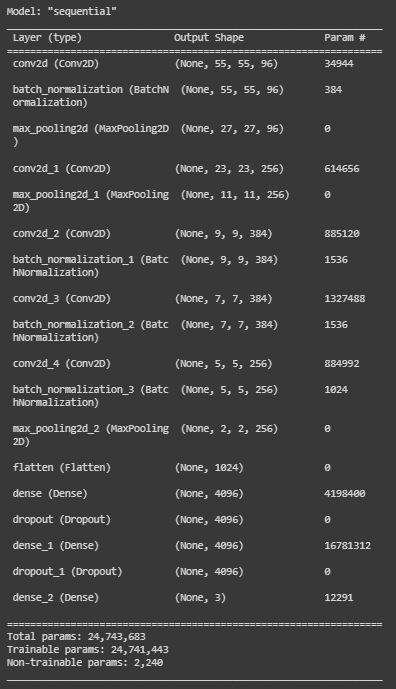
\includegraphics[scale = 1.05]{fileanh/33.jpg}
        \caption{Model Alexnet}
    \end{figure}
\end{center}



\subsubsection{Kết quả training}\newpage
\begin{center}
    \begin{figure}[!h]
        \centering
        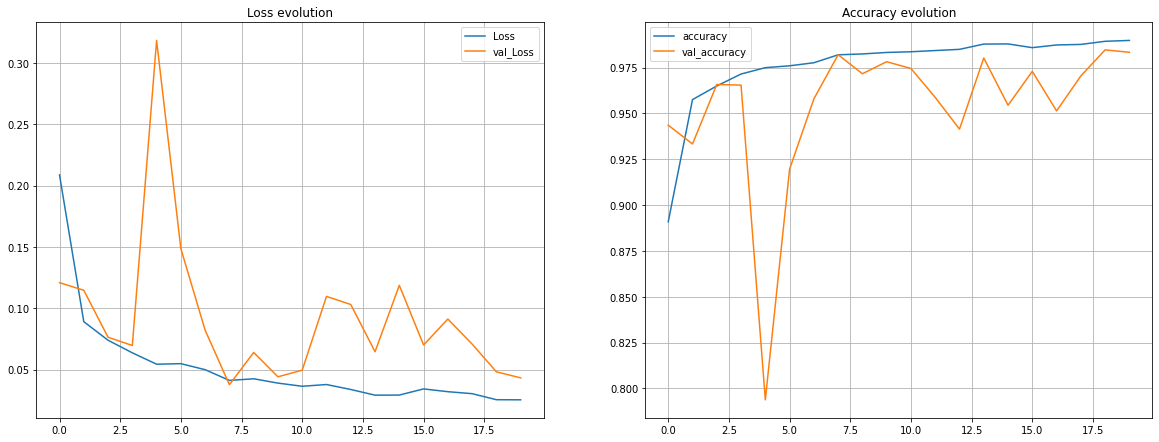
\includegraphics[scale = 0.37]{fileanh/Alexnet.png}
        \caption{kết quả train của Model Alexnet}
    \end{figure}
\end{center}
\subsubsection{Đánh giá}
Các giá trị trên ma trận nhầm lẫn:
%\newpage
\begin{center}
    \begin{figure}[!h]
        \centering
        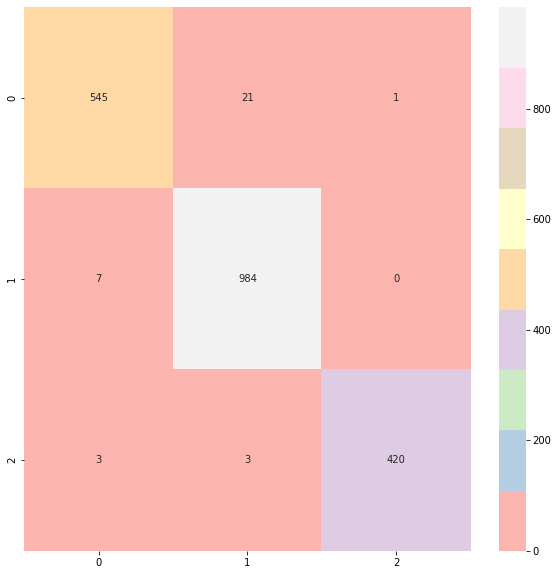
\includegraphics[scale = 0.38]{fileanh/Alexnet1.png}
        \caption{Confusion matrix của Model Alexnet}
    \end{figure}
\end{center}
Và các giá trị Macro average Precision, Macro average Recall, F1-score là:
\begin{center}
    \begin{figure}[!h]
        \centering
        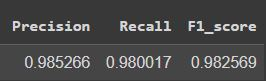
\includegraphics[scale = 1.2]{fileanh/Alexnet2.jpg}
        \caption{Chỉ số đánh giá của Model Alexnet}
    \end{figure}
\end{center}


\subsection{Mô hình 8 - Resnet101}
\subsubsection{Dữ liệu đầu vào}
Bộ dữ liệu \textbf{Fashion Product Images (Small)} đã được xử lý với 41906 hình ảnh cho 3 lớp.
\subsubsection{Xây dựng mô hình}
\begin{lstlisting}
image_size=[227,227]
model=ResNet101(input_shape=image_size+[3],include_top=False,weights="imagenet")
\end{lstlisting}
\begin{lstlisting}
for layers in model.layers:
  layers.trainable=False
\end{lstlisting}
Thêm một số layers cần thiết
\begin{lstlisting}
final_model=Model(inputs=model.input,outputs=Dense(3,activation="softmax")(Flatten()(model.output)))
final_model.summary()
\end{lstlisting}

\begin{center}
    \begin{figure}[!h]
        \centering
        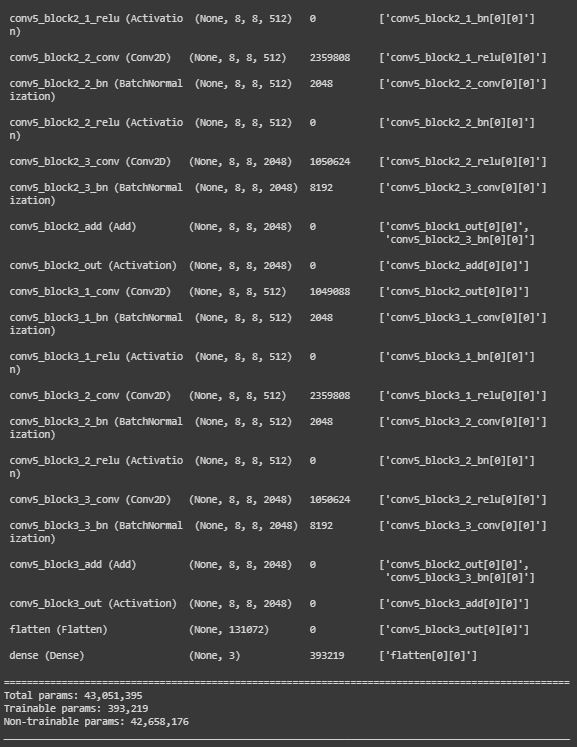
\includegraphics[scale = 0.9]{fileanh/37.jpg}
        \caption{Model Resnet101}
    \end{figure}
\end{center}

\begin{lstlisting}
from tensorflow.keras.optimizers import RMSprop
final_model.compile(loss="categorical_crossentropy",optimizer=RMSprop(lr=0.001),metrics=['accuracy'])
resnet = final_model.fit(training_generator,epochs=50,steps_per_epoch=20,validation_data=validation_generator)
\end{lstlisting}

\subsubsection{Kết quả training}
\begin{center}
    \begin{figure}[!h]
        \centering
        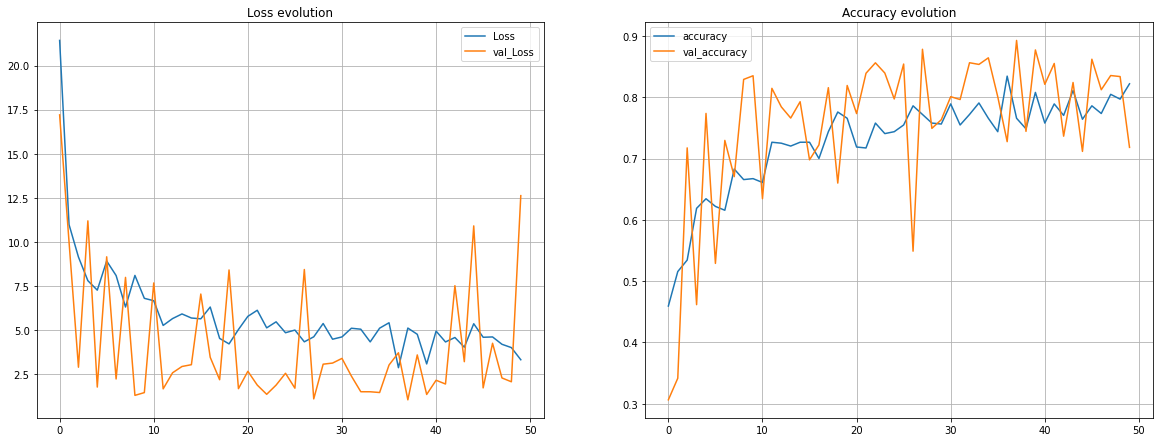
\includegraphics[scale = 0.38]{fileanh/Resnet.png}
        \caption{kết quả train của Model Resnet101}
    \end{figure}
\end{center}
\subsubsection{Đánh giá}
Các giá trị trên ma trận nhầm lẫn:
%\newpage
\begin{center}
    \begin{figure}[!h]
        \centering
        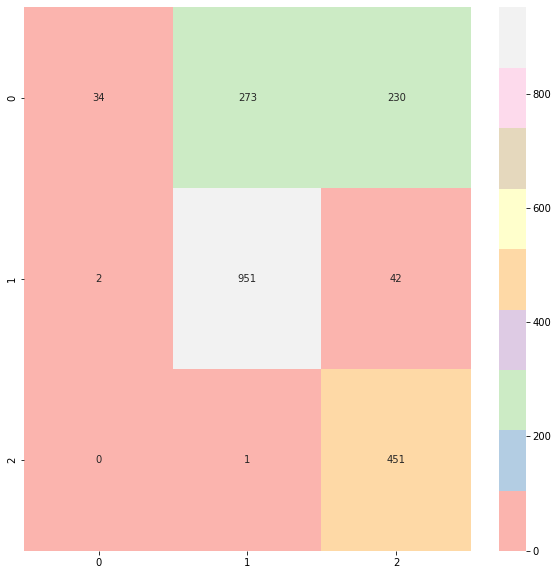
\includegraphics[scale = 0.38]{fileanh/Resnet1.png}
        \caption{Confusion matrix của Model Resnet101}
    \end{figure}
\end{center}
Và các giá trị Macro average Precision, Macro average Recall, F1-score là:
\begin{center}
    \begin{figure}[!h]
        \centering
        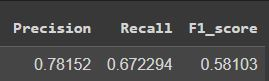
\includegraphics[scale = 1.2]{fileanh/Resnet2.jpg}
        \caption{Chỉ số đánh giá của Model Resnet101}
    \end{figure}
\end{center}

\subsection{Mô hình 9 - Resnet101 với tập dữ liệu lớn}
\subsubsection{Dữ liệu đầu vào }
Bộ dữ liệu đã được tăng cường hình ảnh từ nhiều nguồn khác với tất cả 79596 hình ảnh cho 3 lớp.

\subsubsection{Xây dựng mô hình}
\begin{itemize}
    \item Sử dụng mô hình Resnet101 đã được xây dựng trước đó để thực hiện training với tập dữ liệu lớn hơn.

    \item Đồng thời thực hiện một số thay đổi như sau:
    \begin{itemize}
        \item loss: "categorical\_crossentropy" $\rightarrow$ "binary\_crossentropy"
        
        \item optimizer: RMSprop(lr=0.001) $\rightarrow$ "adam"
    \end{itemize}
    
\end{itemize}
\begin{lstlisting}
final_model.compile(loss="binary_crossentropy",optimizer="adam",metrics=['accuracy'])
\end{lstlisting}


\subsubsection{Kết quả training}
\begin{center}
    \begin{figure}[!h]
        \centering
        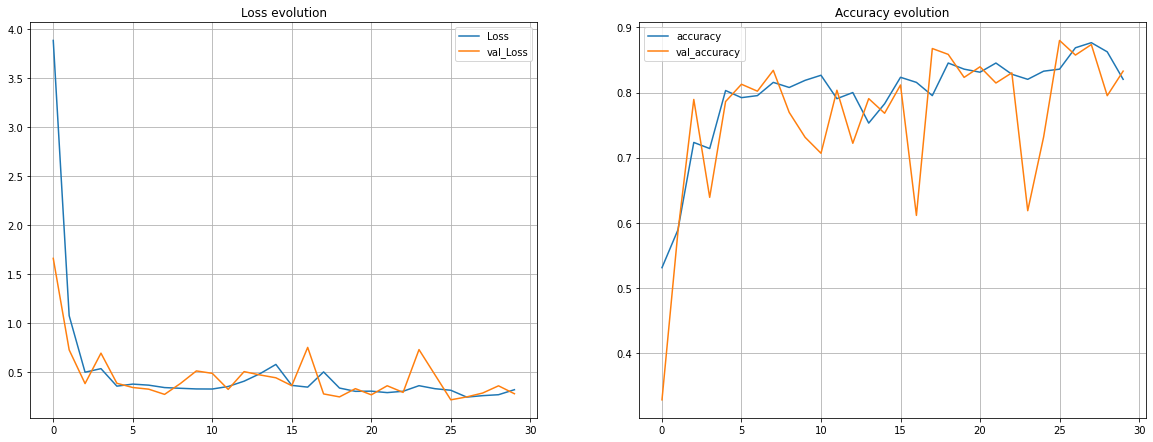
\includegraphics[scale = 0.38]{fileanh/Resnet_increase.png}
        \caption{Kết quả train của Model Resnet101 với tập dữ liệu lớn}
    \end{figure}
\end{center}
\subsubsection{Đánh giá}
Ta có ma trận nhầm lẫn như sau:
\begin{center}
    \begin{figure}[!h]
        \centering
        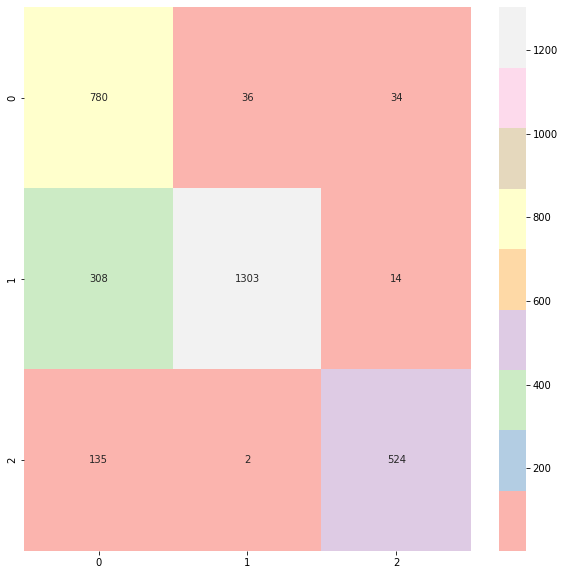
\includegraphics[scale = 0.4]{fileanh/Resnet_increase1.png}
        \caption{Confusion matrix của Model Resnet101 với tập dữ liệu lớn}
    \end{figure}
\end{center}

Và các giá trị Macro average Precision, Macro average Recall, F1-score là:
\begin{center}
    \begin{figure}[!h]
        \centering
        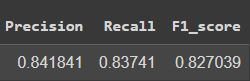
\includegraphics[scale = 1.2]{fileanh/Resnet_increase2.jpg}
        \caption{Các chỉ số đánh giá của Model Resnet101 với tập dữ liệu lớn}
    \end{figure}
\end{center}


\subsection{Mô hình 10 - EfficientNetV2L}
\subsubsection{Dữ liệu đầu vào}
Bộ dữ liệu đã được tăng cường hình ảnh từ nhiều nguồn khác với tất cả 79596 hình ảnh cho 3 lớp.
\subsubsection{Xây dựng mô hình}
\begin{lstlisting}
image_size=[224,224]
model=EfficientNetV2L(input_shape=image_size+[3],include_top=False,weights="imagenet")
\end{lstlisting}
\begin{lstlisting}
for layers in model.layers:
  layers.trainable=False
\end{lstlisting}
Thêm một số layers cần thiết
\begin{lstlisting}
from pandas.core.common import flatten
model=Model(inputs=model.input,outputs=Dense(3,activation="softmax")(Dropout(0.2)(Flatten()(model.output))))
final_model.summary()
\end{lstlisting}

\begin{center}
    \begin{figure}[!h]
        \centering
        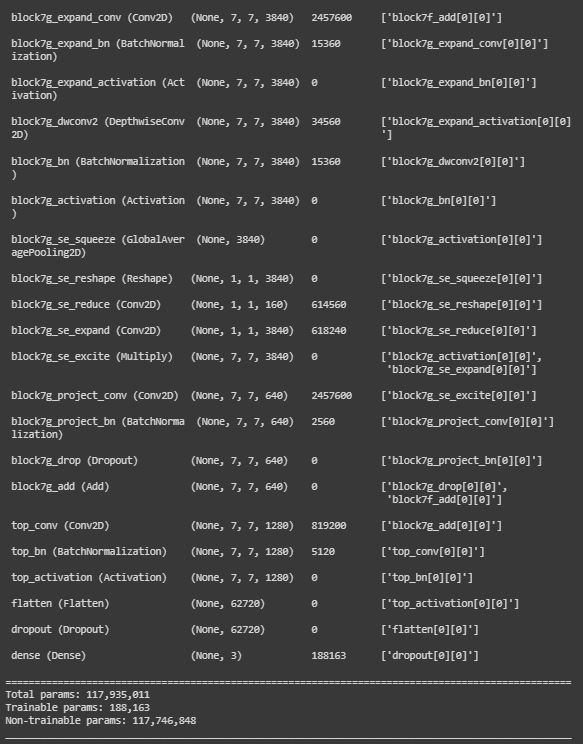
\includegraphics[scale = 1.1]{fileanh/efficient3.jpg}
        \caption{Model EfficientNetV2L}
    \end{figure}
\end{center}

\begin{lstlisting}
model.compile(loss="binary_crossentropy",optimizer="adam",metrics=['accuracy'])
efficientNetV2L = model.fit(training_generator,epochs=30,steps_per_epoch=20,validation_data=validation_generator)
\end{lstlisting}

\subsubsection{Kết quả training}\newpage
\begin{center}
    \begin{figure}[!h]
        \centering
        \includegraphics[scale = 0.38]{fileanh/efficient.png}
        \caption{kết quả train của Model EfficientNetV2L}
    \end{figure}
\end{center}
\subsubsection{Đánh giá}
Các giá trị trên ma trận nhầm lẫn:
%\newpage
\begin{center}
    \begin{figure}[!h]
        \centering
        \includegraphics[scale = 0.38]{fileanh/Resnet1.png}
        \caption{Confusion matrix của Model EfficientNetV2L}
    \end{figure}
\end{center}
Và các giá trị Macro average Precision, Macro average Recall, F1-score là:
\begin{center}
    \begin{figure}[!h]
        \centering
        \includegraphics[scale = 1.2]{fileanh/Resnet2.jpg}
        \caption{Chỉ số đánh giá của Model EfficientNetV2L}
    \end{figure}
\end{center}




    
\newpage
\section{Đóng gói mô hình}
\subsection{Khả năng ứng dụng thực tế}
Với mô hình nhận diện và phân loại các sản phẩm về thời trang này, nếu được phát triển tốt hơn nữa thì nó có thể được đưa vào hệ thống của các trang thương mại điện tử như Shopee, Lazada, ...Ví dụ như khi các nhà bán hàng đăng tải thông tin và hình ảnh của 1 sản phẩm nào đó lên các sàn thương mại, khi đó thay vì phải tự lựa chọn xem chúng thuộc vào loại danh mục nào thì chúng ta chỉ cần tải lên và hệ thống sẽ tự động cập nhật vào danh sách các sản phẩm phù hợp.\\

Ngoài ra, dựa vào kết quả dự đoán của mô hình này thì ta cũng có thể tạo ra một hệ thống gợi ý các sản phẩm tương tự, ví dụ như hình dưới đây:
\begin{center}
    \begin{figure}[!h]
        \centering
        \includegraphics[scale = 0.8]{fileanh/41.jpg}
        \caption{Recommended items}
    \end{figure}
\end{center}


\subsection{Mô hình tiên tiến}
Sử dụng mô hình \textbf{EfficientNetV2L} được trình bày trong paper \href{https://arxiv.org/abs/2104.00298}{\textit{EfficientNetV2: Smaller Models and Faster Training (ICML 2021)}}
\newpage
\input{contents/Chapter cuối}


\end{document} 
